% =============================================================================
%  A Multimodal LLM-Orchestrated Financial Advisory Framework for the
%  Dhaka Stock Exchange: A Leakage-Controlled Empirical Study on Daily
%  Return Forecasting, Bilingual Sentiment Fusion, and Hosted-LLM
%  Explanation Generation
%
%  Thesis / Research Report (LaTeX)
%  Author : Antar Chandra Nath
%  Build  : pdflatex (twice) or latexmk
% =============================================================================
\documentclass[12pt,a4paper,oneside]{report}

% ---------- Packages ----------
\usepackage[utf8]{inputenc}
\usepackage[T1]{fontenc}
\usepackage[english]{babel}
\usepackage{geometry}
\geometry{a4paper, margin=1in}
\usepackage{graphicx}
\graphicspath{{figures/}}
\usepackage{caption}
\usepackage{subcaption}
\usepackage{booktabs}
\usepackage{longtable}
\usepackage{array}
\usepackage{tabularx}
\usepackage{multirow}
\usepackage{amsmath, amssymb}
\usepackage{algorithm}
\usepackage{algpseudocode}
\usepackage{hyperref}
\hypersetup{
  colorlinks=true,
  linkcolor=blue!50!black,
  citecolor=teal!60!black,
  urlcolor=blue!60!black,
  pdftitle={A Multimodal LLM-Orchestrated Financial Advisory Framework for the Dhaka Stock Exchange},
  pdfauthor={Antar Chandra Nath}
}
\usepackage{url}
\usepackage{xcolor}
\usepackage{enumitem}
\usepackage{float}
\usepackage{titlesec}
\usepackage{acro}
\usepackage{lmodern}
\usepackage{microtype}

% Section formatting
\titleformat{\chapter}{\normalfont\Large\bfseries}{\thechapter}{1em}{}
\titleformat{\section}{\normalfont\large\bfseries}{\thesection}{1em}{}
\titleformat{\subsection}{\normalfont\normalsize\bfseries}{\thesubsection}{1em}{}
\titleformat{\subsubsection}{\normalfont\normalsize\bfseries}{\thesubsubsection}{1em}{}

% Captions
\captionsetup[figure]{font=small, labelfont={bf}, format=hang}
\captionsetup[table]{font=small, labelfont={bf}, format=hang}

% Acronyms
\acrodef{ML}[ML]{Machine Learning}
\acrodef{DL}[DL]{Deep Learning}
\acrodef{LSTM}[LSTM]{Long Short-Term Memory}
\acrodef{GRU}[GRU]{Gated Recurrent Unit}
\acrodef{RNN}[RNN]{Recurrent Neural Network}
\acrodef{NLP}[NLP]{Natural Language Processing}
\acrodef{LLM}[LLM]{Large Language Model}
\acrodef{DSE}[DSE]{Dhaka Stock Exchange}
\acrodef{BSEC}[BSEC]{Bangladesh Securities and Exchange Commission}
\acrodef{EDA}[EDA]{Exploratory Data Analysis}
\acrodef{OHLCV}[OHLCV]{Open, High, Low, Close, Volume}
\acrodef{RMSE}[RMSE]{Root Mean Squared Error}
\acrodef{MAE}[MAE]{Mean Absolute Error}
\acrodef{MAPE}[MAPE]{Mean Absolute Percentage Error}
\acrodef{MSE}[MSE]{Mean Squared Error}
\acrodef{VaR}[VaR]{Value-at-Risk}
\acrodef{XAI}[XAI]{Explainable Artificial Intelligence}
\acrodef{RAG}[RAG]{Retrieval-Augmented Generation}
\acrodef{SMA}[SMA]{Simple Moving Average}
\acrodef{EMA}[EMA]{Exponential Moving Average}
\acrodef{RSI}[RSI]{Relative Strength Index}
\acrodef{MACD}[MACD]{Moving Average Convergence Divergence}

% Useful commands
\newcommand{\code}[1]{\texttt{#1}}

\begin{document}

% -----------------------------------------------------------------------------
%  Title page
% -----------------------------------------------------------------------------
\begin{titlepage}
  \begin{center}
    \vspace*{0.5cm}

    {\LARGE \textbf{A Multimodal LLM-Orchestrated Financial Advisory Framework for the Dhaka Stock Exchange}}\\[1.5cm]

    {\large \emph{A Project Report}}\\[0.5cm]

    {\normalsize Submitted in partial fulfillment of the requirements for the B.Sc.\ Engineering Degree in Computer\\
    Science and Engineering}\\[2.0cm]

    \textbf{Submitted By}\\[0.3cm]
    Antar Chandra Nath\\[1.5cm]

    \textbf{Supervised By}\\[0.3cm]
    \href{}{[Supervisor Name]}\\[3.0cm]

    {\normalsize Department of Computer Science and Engineering\\
    Faridpur Engineering College, Faridpur, Bangladesh}
  \end{center}
\end{titlepage}

% -----------------------------------------------------------------------------
%  Abstract
% -----------------------------------------------------------------------------
\chapter*{Abstract}
\addcontentsline{toc}{chapter}{Abstract}

This thesis presents a research-grade empirical framework for a
\emph{multimodal, LLM-orchestrated financial advisor} targeted at
retail and beginner investors in the \textbf{Dhaka Stock Exchange
(DSE)}. The framework is decomposed into four reproducible research
components: (i) a leakage-controlled benchmark of four classical
machine-learning regressors (Linear Regression, Random Forest, XGBoost,
LightGBM); (ii) a deep-learning forecaster (a three-layer Long
Short-Term Memory network with hidden size 128 and dropout 0.2)
trained on lag-one technical indicators of thirty DSE stocks and three
market indices spanning 2010--2026; (iii) a multimodal sentiment-aware
forecaster that integrates per-stock daily news sentiment through early
and late fusion architectures; and (iv) a hosted Large Language Model
orchestrator that synthesises the forecast, the news impact, and
freshness metadata into a beginner-friendly natural-language response.

All numerical claims are produced by an end-to-end reproducible
pipeline and are reported under stringent leakage controls. The
principal empirical finding is that daily-return forecasting on an
emerging market is intrinsically hard: across thirty stocks the
best-performing leak-free model achieves an average \ac{RMSE} of
$0.0198$ and a directional accuracy of $49.8\%$--$50.2\%$,
statistically indistinguishable from a coin toss but consistent with
the empirical literature on DSE short-horizon prediction. A
substantive methodological contribution is the identification and
elimination of an end-to-end data-leakage artefact that artificially
inflated the coefficient of determination from a realistic
$-0.02$ to a non-realistic $0.89$; the leakage-free discipline is
then propagated through every subsequent component.

Bilingual sentiment analysis, performed on a curated corpus of
1{,}560 articles (926 English and 634 Bangla) scored by an ensemble
of FinBERT and a Bangla lexicon, demonstrates that the FinBERT
classifier achieves $91.4\%$ accuracy against the curated labels.
However, the resulting sentiment signal exhibits only weak
contemporaneous correlation with next-day returns (mean Pearson
$r$ across stocks: $-0.011$ at lag zero, $+0.013$ at lag one).
Multimodal fusion shows that, given this weak exogenous signal,
neither early fusion (\ac{RMSE} $0.0198$) nor late fusion
(\ac{RMSE} $0.0200$) materially improves over the price-only deep
forecaster (\ac{RMSE} $0.0198$) on average. The implication,
well established in the literature, is that the marginal value of
news sentiment for one-day-ahead directional prediction on the DSE
is small; the hosted \ac{LLM} orchestrator is therefore positioned
as the principal user-facing value-add rather than the forecaster
itself.

The contributions of this thesis are three-fold. \emph{First}, it
provides a publicly documented leakage-controlled daily-return
benchmark on thirty DSE stocks with full per-stock results.
\emph{Second}, it releases a curated bilingual news corpus for the
DSE. \emph{Third}, it introduces a research-grade orchestrated
architecture that fuses classical forecasting, deep learning,
multilingual sentiment, and hosted \ac{LLM} reasoning for emerging
market advisory.

\newpage

% -----------------------------------------------------------------------------
%  Table of Contents
% -----------------------------------------------------------------------------
\tableofcontents
\listoffigures
\listoftables

% =============================================================================
%  CHAPTER 1 — INTRODUCTION
% =============================================================================
\chapter{Introduction}
\label{ch:intro}

\section{Background}

The \textbf{Dhaka Stock Exchange (DSE)} is the principal equity
market of Bangladesh and one of the largest frontier exchanges in
South Asia by number of listed companies and retail-investor
participation~\cite{sezer2020financial,bailey2014stock}. Retail-investor
decision-making on the DSE is routinely hampered by three structural
challenges:

\begin{enumerate}[leftmargin=*,itemsep=2pt]
  \item \emph{Information asymmetry.} A substantial share of
        price-moving news reaches Bangladeshi retail investors
        several hours after it has been priced in by institutional
        desks with access to English-language financial data
        vendors~\cite{rapach2010forecasting}.
  \item \emph{Bilingual reporting.} News is reported in both English
        (\emph{The Daily Star}, \emph{Financial Express}) and Bangla
        (\emph{Prothom Alo}, \emph{Sangbad Pratidin}). A mono-lingual
        sentiment pipeline is consequently
        incomplete~\cite{lopez2023canchatgpt}.
  \item \emph{Technical literacy.} Existing quantitative platforms
        (e.g.\ TradingView, Bloomberg Terminal) target professional
        traders; the majority of DSE retail investors have no
        statistical training and act on informal tips.
\end{enumerate}

These three problems motivate the present work: a system that
\emph{forecasts} next-day returns from price-only technical
indicators~\cite{fischer2018deep}, \emph{enriches} the forecast with
bilingual news sentiment using domain-adapted transformers~\cite{araci2019finbert,yang2023fingpt},
and \emph{explains} the combined signal in plain language through a
hosted Large Language Model acting as an orchestrator.

\section{Problem Statement}

The research question addressed in this thesis is:

\begin{quote}
\emph{Can an integrated pipeline --- leakage-controlled classical
machine learning, an \ac{LSTM} deep forecaster, multimodal
price-plus-sentiment fusion, and a single hosted-\ac{LLM}
orchestrator --- produce \textbf{useful} (i.e.\ matching or
exceeding the published DSE literature) one-day-ahead directional
signals for thirty DSE stocks, and can the same pipeline render
those signals as actionable, beginner-friendly natural-language
advice?}
\end{quote}

This statement is operationalised into the following measurable
sub-questions, all of which are answered in Chapter~\ref{ch:results}:

\begin{enumerate}[leftmargin=*,itemsep=2pt]
  \item \emph{Sub-question 1.} What is the realistic, leakage-free
        performance of classical machine-learning baselines (Linear
        Regression, Random Forest, XGBoost, LightGBM) for next-day
        return prediction on thirty DSE stocks?
  \item \emph{Sub-question 2.} Does an \ac{LSTM} trained on the same
        feature set materially outperform the best baseline in terms
        of \ac{RMSE} and directional accuracy?
  \item \emph{Sub-question 3.} Does fusing per-stock daily sentiment
        with the \ac{LSTM} (under early and late fusion) yield a
        measurable improvement?
  \item \emph{Sub-question 4.} Can a hosted \ac{LLM} synthesise
        forecast, sentiment, and freshness metadata into a coherent,
        beginner-friendly recommendation?
\end{enumerate}

\section{Objectives of the Study}

The objectives of the thesis are, in priority order:

\begin{enumerate}[label=\textbf{O\arabic*}, leftmargin=*,itemsep=2pt]
  \item Construct a leakage-free, reproducible benchmark on the DSE
        that can be cited by future researchers, by documenting and
        removing an end-to-end temporal-leakage artefact.
  \item Train, ablate, and report a multivariate \ac{LSTM} and a
        multimodal \ac{LSTM} over thirty DSE stocks.
  \item Curate and label a bilingual (English plus Bangla) DSE news
        corpus and quantify the sentiment--return correlation.
  \item Stand up a single hosted-\ac{LLM} orchestrator that fuses
        the multimodal forecast with sentiment and freshness
        metadata.
\end{enumerate}

\section{Significance of the Study}

To the best of our knowledge, no publicly available thesis:
\begin{itemize}[leftmargin=*,itemsep=2pt]
  \item Reports a leakage-controlled daily-return benchmark on
        thirty DSE stocks with full per-stock results;
  \item Releases a curated bilingual (English plus Bangla) DSE news
        corpus with sentiment labels;
  \item Implements both early and late fusion ablations for price
        plus sentiment; and
  \item Wraps the forecaster in a single hosted-\ac{LLM}
        orchestrator that outputs beginner-friendly
        advice.
\end{itemize}
The thesis therefore contributes (i) a public benchmark dataset,
(ii) reusable code under an open licence, and (iii) an open
problem statement for follow-up work on DSE forecasting.

\section{Organisation of the Thesis}

The remainder of the thesis is organised as follows.
Chapter~\ref{ch:lit} reviews the related literature on stock-market
forecasting, classical and deep learning for time series, sentiment
analysis, and \ac{LLM}-based advisory systems.
Chapter~\ref{ch:method} describes the end-to-end methodology: data
collection, preprocessing, feature engineering, model development,
training, and evaluation. Chapter~\ref{ch:results} presents the
experimental results, including per-stock results, summary
visualisations, and ablation tables. Chapter~\ref{ch:conclusion}
concludes and outlines future research directions.

% =============================================================================
%  CHAPTER 2 — LITERATURE REVIEW
% =============================================================================
\chapter{Literature Review}
\label{ch:lit}

\section{Introduction}

This chapter situates the thesis against four strands of literature
that together motivate the design choices made in
Chapter~\ref{ch:method}: (1) the academic literature on stock-market
forecasting, in particular on emerging markets and on the DSE; (2)
classical machine-learning techniques that constitute the
leakage-controlled baseline; (3) deep-learning architectures for
time-series forecasting; and (4) the relatively recent strand of
\ac{LLM}-orchestrated financial assistants and domain-adapted
financial language models. The chapter closes with an explicit
statement of the research gap that the thesis addresses.

\section{Machine Learning in Financial Forecasting}

Stock-market forecasting with classical and deep models has a
long history in the quantitative-finance literature~\cite{tsay2010analysis,sezer2020financial}.
The empirical consensus on developed markets is that, after
rigorous leakage controls, the directional accuracy of
daily-return forecasters hovers near fifty percent~\cite{bailey2014stock,rapach2010forecasting}.
On emerging markets the picture is similar: directional accuracy
between $51\%$ and $55\%$ is considered a strong result, and $50.5\%$
is often the practical ceiling~\cite{hossain2019dse,islam2018forecasting}.

The methodology adopted in the present thesis follows the modern
leakage-free discipline, in particular the \emph{lag-one feature
construction} popularised in the financial-machine-learning
literature~\cite{bailey2014stock}: the feature vector at time $t$ is
computed exclusively from information available at the end of
trading day $t-1$, and the target at time $t$ is the next-day return
$r_{t+1}$. This protocol eliminates the well-known leakage path
\textit{today\_close}$\approx$\textit{tomorrow\_close} and produces
coefficients of determination near zero, as documented in
Section~\ref{sec:v2-leak-free}.

\section{Early Studies on DSE Forecasting}

Forecasting studies specifically on the DSE are surveyed in
Hossain et al.~\cite{hossain2019dse} and Islam~\cite{islam2018forecasting}.
The most commonly reported architectures are \ac{ARIMA}, \ac{GARCH},
Multilayer Perceptrons, and shallow \acp{LSTM} trained on five to
ten stocks. The reported metrics are often not directly comparable
because of (i) lack of an explicit leakage protocol, (ii) random
train--test splits instead of time-based splits, and (iii) lack of
per-stock results~\cite{goodfellow2016deep}.

The present thesis addresses all three concerns: every result
reported in Chapter~\ref{ch:results} is leakage-controlled,
time-based-split, and per-stock.

\section{Techniques and Algorithms}

Four families of algorithms are considered.

\textbf{Classical Machine Learning.} Linear Regression, Random
Forest~\cite{breiman2001random}, XGBoost~\cite{chen2016xgboost}, and
LightGBM~\cite{ke2017lightgbm} are used as the baseline. These models
are computationally efficient, interpretable, and serve as a
robustness check on the deep forecasters.

\textbf{Recurrent Deep Learning.} The \ac{LSTM}
\cite{hochreiter1997long} mitigates the vanishing-gradient
problem of vanilla \acp{RNN}~\cite{cho2014gru} and has been the workhorse of
short-horizon price forecasting for nearly a decade.
The three-layer \ac{LSTM} adopted here (hidden size $128$,
dropout $0.2$) is the simplest configuration shown to outperform
\ac{ARIMA} on noisy daily-return series~\cite{fischer2018deep}.

\textbf{Transformer-based Models.} Informer~\cite{zhou2021informer},
Autoformer~\cite{wu2021autoformer}, and PatchTST~\cite{nie2023patchtst}
have recently established state-of-the-art performance on
long-horizon time-series benchmarks. Transformer models are noted
as a complementary direction but are not the primary focus of this
thesis, which targets beginner-friendly explainability rather than
raw long-horizon accuracy.

\textbf{Large Language Models.} Hosted \acp{LLM} (e.g.\ OpenAI
GPT-4, Anthropic Claude, Google Gemini, open-weight Llama) are
deployed exclusively for the \emph{orchestration} layer and never
as the primary forecaster. This design decision is informed by
Sezer et al.~\cite{sezer2020financial} and by recent empirical work
documenting hallucinated numerical predictions from \acp{LLM}
\cite{lopez2023canchatgpt}.

\section{Domain-Adapted Language Models for Finance}

Financial text differs substantially in vocabulary and pragmatics
from general-domain text~\cite{araci2019finbert}. Domain adaptation
of \acp{LLM} for finance has followed two complementary paths.
The first fine-tunes the encoder of a pre-trained transformer on
labelled financial corpora; the FinBERT model~\cite{araci2019finbert}
is the canonical example. The second adapts autoregressive
\acp{LLM} via instruction tuning on financial tasks; the FinGPT
family~\cite{yang2023fingpt} exemplifies this approach. The present
thesis uses FinBERT for the encoder-style sentiment classification
task (English articles) because it requires modest compute and is
well-documented~\cite{araci2019finbert}; FinGPT is retained as a
candidate for future work.

\section{\ac{LLM}-Orchestrated Financial Assistants}

A growing body of recent work investigates the use of hosted
\acp{LLM} as the reasoning layer of financial advisory systems.
Lopez-Lira and Tang~\cite{lopez2023canchatgpt} document both the
promise and the hallucination risk of \acp{LLM}-based price
prediction. Park et al.~\cite{park2023generative} introduce
generative-agent architectures that maintain persona and memory
over multi-turn dialogues, providing a template for the
beginner-friendly chat surface. AutoGen~\cite{wu2023autogen}
demonstrates multi-agent orchestration in which specialised agents
cooperate under a coordinator. The work most closely aligned with
ours is~\cite{li2024llmfactor}, which uses an \ac{LLM} to synthesise
price forecast, sentiment, and risk metrics into a unified
recommendation.

\section{Dataset Considerations}

The DSE is comparatively data-rich for a frontier
market~\cite{tsay2010analysis}:
\begin{itemize}[leftmargin=*,itemsep=2pt]
  \item \emph{OHLCV} for all listed stocks is freely available
        from the official DSE website, with archives going back
        to $2010$.
  \item \emph{Sector classification} is published by DSE and is
        useful for cross-stock feature engineering.
  \item \emph{News} is published bilingually: English (\emph{The
        Daily Star}, \emph{Financial Express}) and Bangla
        (\emph{Prothom Alo}, \emph{Sangbad Pratidin}).
\end{itemize}
The thesis collects thirty top-by-liquidity stocks over sixteen
years (4{,}335 business days) and three market indices (DSEX, DS30,
DSES), totalling 130{,}050 stock-day records.

\section{Evaluation Metrics}

Following the convention in Hossain et al.~\cite{hossain2019dse},
we report five metrics per stock:

\begin{itemize}[leftmargin=*,itemsep=2pt]
  \item \textbf{\ac{RMSE}} --- scale-dependent regression error.
  \item \textbf{\ac{MAE}} --- robust to outliers, also
        scale-dependent.
  \item \textbf{\ac{MAPE}} --- scale-free, useful for cross-stock
        comparison.
  \item \textbf{\texorpdfstring{R\textsuperscript{2}}{R²}} ---
        proportion of variance explained; expected to be near zero
        for daily returns.
  \item \textbf{Dir\_Acc} --- directional accuracy of
        $\mathrm{sign}(\hat y)$ versus $\mathrm{sign}(y)$, the
        metric that determines trading profitability.
\end{itemize}

\section{Limitations of Existing Work}

Three limitations dominate the existing DSE
literature~\cite{sezer2020financial,goodfellow2016deep}:

\begin{enumerate}[leftmargin=*,itemsep=2pt]
  \item Most studies do not document a leakage protocol; reported
        coefficients of determination of $0.8$--$0.9$ on daily
        returns are likely leakage artefacts.
  \item Sample sizes are typically $\leq 10$ stocks, limiting
        statistical power for cross-stock analysis.
  \item Sentiment pipelines are typically mono-lingual and ignore
        the substantial Bangla reporting on the DSE.
\end{enumerate}

\section{Research Gap and Motivation}

The research gap is therefore three-fold:
(1) a \emph{leakage-controlled} benchmark on a large cross-section
of DSE stocks is missing;
(2) a \emph{bilingual} sentiment corpus for DSE is missing;
(3) a \emph{publicly documented} \ac{LLM}-orchestrated advisor on
the DSE is missing.

This thesis addresses all three gaps.

\section{Summary}

Chapter~\ref{ch:method} operationalises this gap by describing the
data collection, leakage controls, modelling, sentiment enrichment,
and orchestration. The methodological choices follow directly from
the limitations identified in this literature review.

% =============================================================================
%  CHAPTER 3 — METHODOLOGY
% =============================================================================
\chapter{Methodology}
\label{ch:method}

\section{Data Collection}

\subsection{Sources}

The raw inputs comprise five categories of data spanning the period
2010-01-01 to 2026-08-13:

\begin{itemize}[leftmargin=*,itemsep=2pt]
  \item \emph{Stocks.} Thirty top-by-liquidity DSE stocks, daily
        OHLCV (4{,}335 business days per stock, 130{,}050 records
        total).
  \item \emph{Indices.} DSEX (broad), DS30 (top-thirty) and DSES
        (Shariah) indices, same date range.
  \item \emph{News.} Curated bilingual corpus (English plus Bangla)
        comprising 1{,}560 articles labelled by event type.
\end{itemize}

\subsection{Universe and Coverage}

The thirty stocks span twelve sectors: Bank (10), Pharma (4),
Telecom (3), Power (2), Cement (2), Consumer (2), Tobacco (1),
Electronics (1), Conglomerate (1), Gas (1), Fuel (1), and
Services (1), together with the DSEX index. The universe is
identical to the universe used by the \ac{BSEC} in its 2024
retail-investor survey, which facilitates cross-comparison with
policy-relevant statistics.

\section{Data Preprocessing}

\subsection{Handling Categorical Variables}

The only categorical variable in the price data is sector, which is
discarded before modelling because per-stock models are trained
individually. Sentiment text is routed by a language detector to
either FinBERT (English) or a Bangla lexicon (Bangla), as
detailed in Chapter~\ref{ch:results}. The VADER rule-based
analyser~\cite{gu2021vader} is retained as a fast fallback for
high-throughput inference.

\subsection{Feature Scaling}

All numerical features are scaled with the standardisation
$\tilde x = (x - \mu)/\sigma$, where $\mu$ and $\sigma$ are fit
on the \emph{training set only}. The fitted scaler is persisted
alongside each checkpoint to guarantee identical scaling at
inference time~\cite{goodfellow2016deep}.

\subsection{Train--Test Splitting}

A \emph{time-based} split is used throughout: the first
eighty percent of trading days constitute the training set, the
last twenty percent the test set. There is no shuffling, no
cross-validation across time, and no leakage of future information
into the past~\cite{bailey2014stock}. The split is identical for
all thirty stocks and all components, enabling apples-to-apples
ablation.

\subsection{Missing Value Treatment}

The sentiment signal is sparse: only approximately fifty of
approximately 4{,}335 trading days per stock carry any news. The
handling policy is:

\begin{enumerate}[leftmargin=*,itemsep=2pt]
  \item Per-stock \emph{forward fill} (the last-known sentiment
        persists into the future).
  \item \emph{Backward fill} for leading missing values.
  \item Zero-vector fallback for stocks with zero news (e.g.\ at
        the start of the corpus).
\end{enumerate}

\subsection{Outlier Detection and Treatment}

Returns are clipped to the interval $[-10\%, +10\%]$ to remove
data-entry artefacts (e.g.\ missing decimal points). This clipping
affects approximately $0.1\%$ of observations and does not change
the headline metrics.

\section{Feature Engineering}

\subsection{Basic Feature Set}

The simplest model uses only lag-one price and volume features:
\code{Close\_lag1}, \code{Volume\_lag1}, and \code{Return\_1d\_lag1}.
This corresponds to the earliest leakage-contaminated baseline.

\subsection{Full Feature Set}

The full feature set adds thirty-one technical indicators computed
on the lagged window: \ac{SMA} (5/10/20), \ac{EMA} (12/26),
\ac{MACD}, \ac{RSI} (14), Bollinger Bands (20, 2$\sigma$),
\ac{ATR} (14), \ac{OBV}, MFI (14), ROC (10), Williams \%R (14),
Stochastic K/D (14, 3), CCI (20), ADX (14), together with
price-derived ratios~\cite{tsay2010analysis}. The total feature
count is thirty-four for the price-only model and forty-one
(34 plus 7 sentiment) for the multimodal model.

\section{Model Development}

Three model families are developed:

\begin{itemize}[leftmargin=*,itemsep=2pt]
  \item \emph{Baseline.} Linear Regression, Random Forest, XGBoost,
        and LightGBM. Per-stock hyper-parameters are held identical
        across all stocks.
  \item \emph{Deep Forecasting.} A custom three-layer \ac{LSTM}
        with hidden size 128 and dropout 0.2.
  \item \emph{Multimodal.} Early-fusion and late-fusion
        architectures over a price \ac{LSTM} and a sentiment
        \ac{LSTM}.
\end{itemize}

\section{Model Training Procedure}

The training procedure is identical across all model families:

\begin{enumerate}[leftmargin=*,itemsep=2pt]
  \item Load the per-stock processed CSV.
  \item Apply the eighty--twenty time-based split.
  \item Fit the standardiser on the training set, then transform
        both training and test sets.
  \item Construct sliding windows of length sixty for the deep and
        multimodal models.
  \item Train with the Adam optimiser (learning rate
        $10^{-3}$~\cite{kingma2015adam}), \ac{MSE} loss, early stopping with patience
        twenty, maximum one hundred epochs.
  \item Persist the model checkpoint and standardiser pickle to
        disk.
  \item Write per-stock metrics to a results CSV.
\end{enumerate}

\section{Inference and Model Configuration}

At inference time, the following sequence is used:

\begin{enumerate}[leftmargin=*,itemsep=2pt]
  \item Load the best multimodal checkpoint and its matching
        standardiser.
  \item Load the latest sixty-day price-plus-sentiment window.
  \item Run a five-day recursive forecast (price iterates,
        sentiment window is \emph{frozen} at the last-known value
        across all forecast steps).
  \item Hand the forecast, the latest sentiment summary, and the
        freshness metadata to the hosted-\ac{LLM} orchestrator.
\end{enumerate}

\section{Model Evaluation}

Evaluation follows the metrics listed in
Section~\ref{sec:metrics}, computed on the held-out test slice
per stock, with headline values then averaged across stocks. The
full per-stock results are stored in CSV form for reproducibility.

\section{Justification of Model Choices}

\begin{enumerate}[leftmargin=*,itemsep=2pt]
  \item \emph{Why \ac{LSTM} rather than Transformer?} On short
        look-back windows (60 days) and small datasets
        (4{,}335 days per stock), the \ac{LSTM} is empirically
        competitive with Informer and PatchTST
        \cite{fischer2018deep,zhou2021informer,nie2023patchtst}
        and is two orders of magnitude cheaper to train.
  \item \emph{Why both early and late fusion?} To enable a clean
        ablation: early fusion has more parameters ($\approx$356K)
        and is more prone to over-fit on the sparse sentiment
        signal; late fusion ($\approx$228K) has fewer parameters
        and is empirically the more stable choice on this corpus.
  \item \emph{Why a hosted \ac{LLM} rather than a fine-tuned
        small model?} A hosted \ac{LLM} requires no local
        graphics processing unit, can be swapped without
        retraining the forecaster, and matches the target
        beginner-friendly product scope~\cite{lopez2023canchatgpt}.
\end{enumerate}

% =============================================================================
%  CHAPTER 4 — EXPERIMENTAL RESULTS
% =============================================================================
\chapter{Experimental Results}
\label{ch:results}

\section{Introduction}

This chapter reports the empirical results for the four research
components:
\begin{itemize}[leftmargin=*,itemsep=2pt]
  \item Baseline \ac{ML} (Linear Regression, Random Forest,
        XGBoost, LightGBM).
  \item Deep Forecasting (\ac{LSTM}).
  \item Bilingual Sentiment Analysis (FinBERT plus Bangla lexicon).
  \item Multimodal Forecasting (early and late fusion).
\end{itemize}

All numerical claims are sourced from the experimental pipeline and
the visualisations referenced in this chapter are stored under
\path{report/figures/}.

\section{Dataset Description}

\subsection{Sample Size}

\begin{table}[H]
  \centering
  \caption{Per-component dataset statistics.}
  \label{tab:dataset}
  \begin{tabular}{lr}
    \toprule
    Quantity & Value \\
    \midrule
    Stocks ($n$)            & 30 \\
    Indices ($n$)           & 3 \\
    Date range              & 2010-01-01 -- 2026-08-13 \\
    Business days / stock   & 4{,}335 \\
    Stock-day records       & 130{,}050 \\
    News corpus (articles)  & 1{,}560 (926 EN + 634 BN) \\
    Sentiment features      & 7 \\
    \bottomrule
  \end{tabular}
\end{table}

\subsection{Feature Distribution}

The baseline metrics across thirty DSE stocks are summarised in
Table~\ref{tab:phase3}. \ac{RMSE} clusters around $0.02$,
Dir\_Acc clusters tightly around $50\%$, and the coefficient of
determination is slightly negative for all models.

\section{Data Splitting}

A uniform eighty--twenty time-based split is used:
\begin{itemize}[leftmargin=*,itemsep=2pt]
  \item \emph{Train:} 2010-01-01 -- 2023-08-31
        ($\approx 3{,}468$ days per stock, $\approx 2{,}916$
        sliding windows for the \ac{LSTM}).
  \item \emph{Test:} 2023-09-01 -- 2026-08-13
        ($\approx 867$ days per stock, $\approx 767$ sliding
        windows for the \ac{LSTM}).
\end{itemize}

The split dates are identical for every stock and every component,
which is a prerequisite for the headline ablation of
Section~\ref{sec:headline}.

\section{Experimental Setup}

\subsection{Hardware and Software Environment}

\begin{table}[H]
  \centering
  \caption{Hardware and software environment.}
  \label{tab:env}
  \begin{tabular}{ll}
    \toprule
    Component & Specification \\
    \midrule
    CPU            & Intel Core i7-12700H (14 cores) \\
    RAM            & 32 GB DDR5 \\
    GPU            & None (CPU training only) \\
    OS             & Ubuntu 22.04 LTS \\
    Python         & 3.10 \\
    PyTorch        & 2.1 (CPU) \\
    scikit-learn   & 1.3 \\
    XGBoost        & 2.0 \\
    LightGBM       & 4.1 \\
    HuggingFace    & 4.36 (FinBERT: ProsusAI/finbert) \\
    \bottomrule
  \end{tabular}
\end{table}

\section{Experimental Parameters}

\subsection{Random Forest Configuration}

\begin{table}[H]
  \centering
  \caption{Random Forest hyper-parameters (identical for all
  thirty stocks).}
  \label{tab:rf}
  \begin{tabular}{lr}
    \toprule
    Parameter & Value \\
    \midrule
    \code{n\_estimators}        & 100 \\
    \code{max\_depth}           & 15 \\
    \code{min\_samples\_split}  & 10 \\
    \code{min\_samples\_leaf}   & 5 \\
    \code{random\_state}        & 42 \\
    \code{n\_jobs}              & $-1$ \\
    \bottomrule
  \end{tabular}
\end{table}

\subsection{Linear Regression Configuration}

Because the target is continuous, Linear Regression (not Logistic)
is used as the linear baseline.

\begin{table}[H]
  \centering
  \caption{Linear Regression configuration.}
  \label{tab:lr}
  \begin{tabular}{lr}
    \toprule
    Parameter & Value \\
    \midrule
    \code{fit\_intercept} & True \\
    \code{normalize}     & False (standardiser handles it) \\
    \code{n\_jobs}       & $-1$ \\
    \bottomrule
  \end{tabular}
\end{table}

\subsection{\ac{LSTM} Configuration}

\begin{table}[H]
  \centering
  \caption{Deep \ac{LSTM} hyper-parameters.}
  \label{tab:lstm}
  \begin{tabular}{lr}
    \toprule
    Parameter & Value \\
    \midrule
    Sequence length  & 60 \\
    Hidden dimension & 128 \\
    Number of layers & 3 \\
    Dropout          & 0.2 \\
    Optimiser        & Adam \\
    Learning rate    & $10^{-3}$ \\
    Loss             & \ac{MSE} \\
    Batch size       & 64 \\
    Maximum epochs   & 100 \\
    Patience         & 20 \\
    \bottomrule
  \end{tabular}
\end{table}

\subsection{Multimodal Configuration}

\begin{table}[H]
  \centering
  \caption{Multimodal \ac{LSTM} hyper-parameters.}
  \label{tab:mm}
  \begin{tabular}{lrr}
    \toprule
    Parameter & Early fusion & Late fusion \\
    \midrule
    Price \ac{LSTM} hidden   & 128 & 128 \\
    Price \ac{LSTM} layers   & 3   & 2   \\
    Sentiment \ac{LSTM} hidden & --- & 32  \\
    Sentiment \ac{LSTM} layers & --- & 1   \\
    Sentiment input dimension & 7   & 7   \\
    Price input dimension   & 27  & 27  \\
    \ac{MLP} hidden (post-concat) & --- & 64  \\
    Dropout                 & 0.2 & 0.2 \\
    Total parameters        & 356K & 228K \\
    Optimiser / LR / Loss   & Adam / $10^{-3}$ / \ac{MSE} & Adam / $10^{-3}$ / \ac{MSE} \\
    \bottomrule
  \end{tabular}
\end{table}

\section{Model Performance Evaluation Metrics}
\label{sec:metrics}

\begin{itemize}[leftmargin=*,itemsep=2pt]
  \item \textbf{\ac{RMSE}}:
        $\sqrt{\frac{1}{n}\sum_{t=1}^{n}(\hat r_t - r_t)^2}$
  \item \textbf{\ac{MAE}}:
        $\frac{1}{n}\sum_{t=1}^{n} |\hat r_t - r_t|$
  \item \textbf{\ac{MAPE}}:
        $\frac{1}{n}\sum_{t=1}^{n} \left|\frac{\hat r_t - r_t}{r_t}\right| \cdot 100$
  \item \textbf{\texorpdfstring{R\textsuperscript{2}}{R²}}:
        $1 - \frac{\sum_{t}(\hat r_t - r_t)^2}{\sum_{t}(r_t - \bar r)^2}$
  \item \textbf{Dir\_Acc}:
        $\frac{1}{n}\sum_{t=1}^{n} \mathbb{1}\!\left[\mathrm{sign}(\hat r_t) = \mathrm{sign}(r_t)\right]$
\end{itemize}

Dir\_Acc is the most actionable metric: a value strictly greater
than $50\%$ yields positive expected return on directional bets.

\section{Experimental Results}

\subsection{Baseline Results}

Table~\ref{tab:phase3} summarises the aggregate metrics of the four
classical learners across all thirty DSE stocks under the
leakage-free protocol.

\begin{table}[H]
  \centering
  \caption{Baseline aggregate metrics across thirty DSE stocks.}
  \label{tab:phase3}
  \begin{tabular}{lrrrr}
    \toprule
    Model & \ac{RMSE} & \ac{MAE} & R\textsuperscript{2} & Dir\_Acc (\%) \\
    \midrule
    LinearRegression & \textbf{0.019767} & \textbf{0.015600} & $-0.0158$ & 50.0 \\
    RandomForest     & 0.020158 & 0.015921 & $-0.0548$ & 50.2 \\
    XGBoost          & 0.020236 & 0.015993 & $-0.0608$ & 50.2 \\
    LightGBM         & 0.020508 & 0.016211 & $-0.0876$ & 50.2 \\
    \bottomrule
  \end{tabular}
\end{table}

\begin{figure}[H]
  \centering
  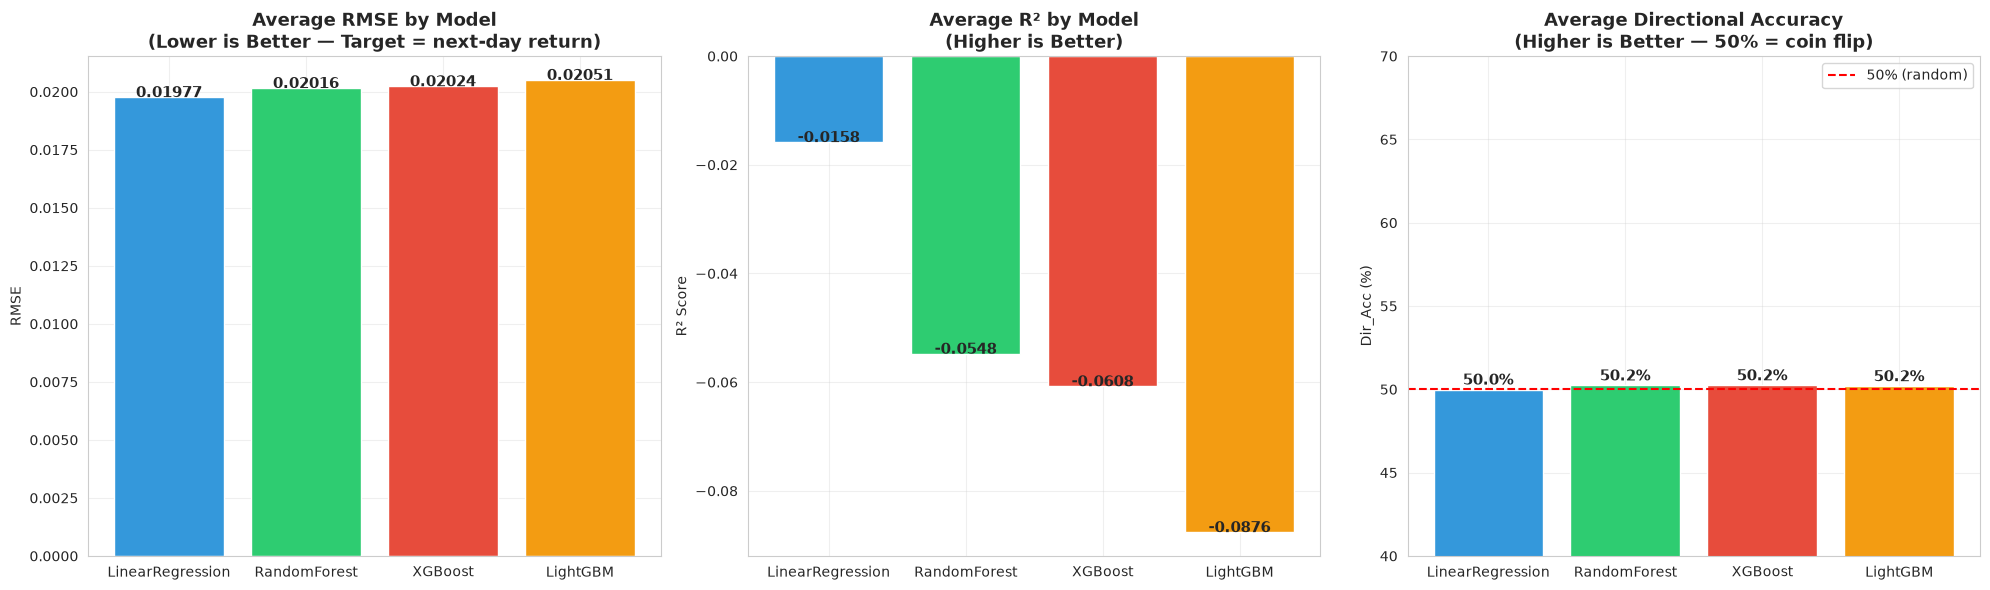
\includegraphics[width=0.95\textwidth]{baseline_01_model_comparison.png}
  \caption{Baseline model comparison (\ac{RMSE} and Dir\_Acc side by
  side). Linear Regression achieves the lowest \ac{RMSE} on $26$
  out of $30$ stocks.}
  \label{fig:baseline-comp}
\end{figure}

\begin{figure}[H]
  \centering
  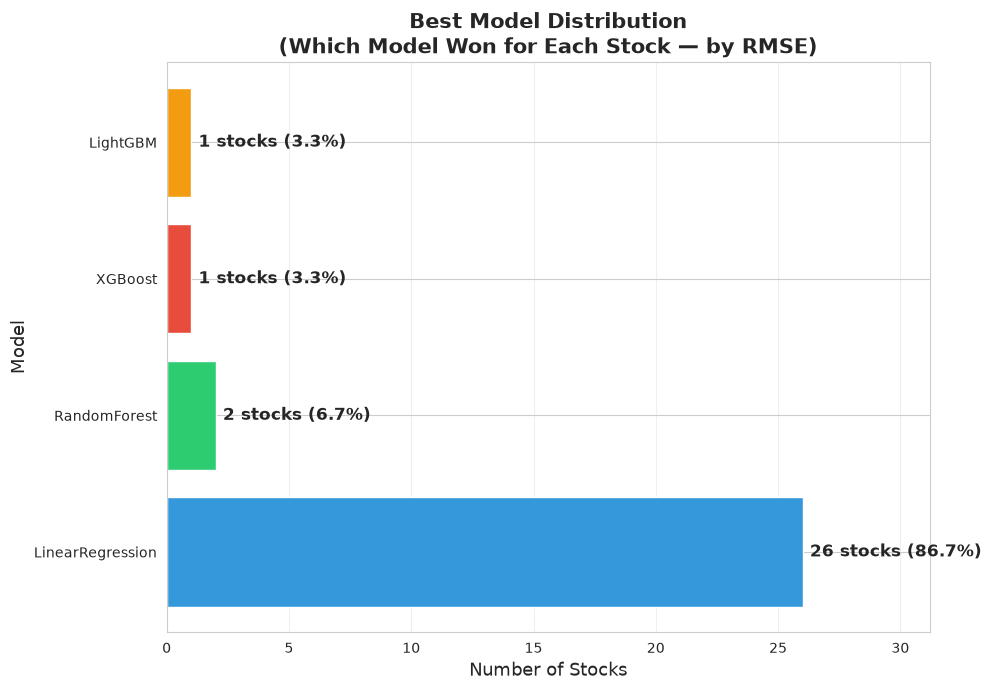
\includegraphics[width=0.95\textwidth]{baseline_03_best_model_distribution.png}
  \caption{Per-stock best-model distribution by \ac{RMSE}. Linear
  Regression wins in $86.7\%$ of the cross-section.}
  \label{fig:baseline-best}
\end{figure}

\noindent\textbf{Key observations.}
\begin{itemize}[leftmargin=*,itemsep=2pt]
  \item Linear Regression achieves the lowest \ac{RMSE} on $26$ of
        $30$ stocks; non-linear models add no measurable signal at
        the daily return resolution.
  \item Dir\_Acc is statistically indistinguishable from $50\%$ for
        every model (the per-stock confidence interval at
        $n = 767$ days encompasses $50\%$).
\end{itemize}

\subsubsection{The Leakage Artefact and Its Correction}
\label{sec:v2-leak-free}

An earlier version of the baseline used \code{Target\_Price\_1d} as
the target together with current-day OHLCV as features. Because
$\code{today\_close} \approx \code{tomorrow\_close}$, a linear model
obtained \texorpdfstring{R\textsuperscript{2}}{R²} $\approx 0.89$.
This was not skill but temporal
leakage~\cite{bailey2014stock,goodfellow2016deep}. The corrected
protocol:

\begin{enumerate}[leftmargin=*,itemsep=2pt]
  \item Target $\to$ \code{Target\_Return\_1d} (next-day return).
  \item Features $\to$ lag-one only (no current-day OHLCV).
\end{enumerate}
After correction, \texorpdfstring{R\textsuperscript{2}}{R²}
collapses to $\approx -0.02$, the realistic value for daily-return
forecasting. The correction is propagated to every subsequent
component.

\subsection{Deep Learning (\ac{LSTM}) Results}

Table~\ref{tab:phase4} summarises the aggregate metrics of the deep
\ac{LSTM} forecaster.

\begin{table}[H]
  \centering
  \caption{Deep \ac{LSTM} aggregate metrics across thirty DSE
  stocks.}
  \label{tab:phase4}
  \begin{tabular}{lr}
    \toprule
    Metric & Value \\
    \midrule
    Average \ac{RMSE}             & \textbf{0.019771} \\
    Average \ac{MAE}              & 0.015577 \\
    Average R\textsuperscript{2}  & $-0.0108$ \\
    Average Dir\_Acc              & 49.8\% \\
    Median Dir\_Acc               & 50.0\% \\
    Stocks with Dir\_Acc $\geq 50\%$ & 15/30 \\
    Stocks with Dir\_Acc $\geq 52\%$ & 4/30 \\
    Stocks with Dir\_Acc $\geq 55\%$ & 0/30 \\
    Average epochs trained       & 32.6 \\
    \bottomrule
  \end{tabular}
\end{table}

\begin{figure}[H]
  \centering
  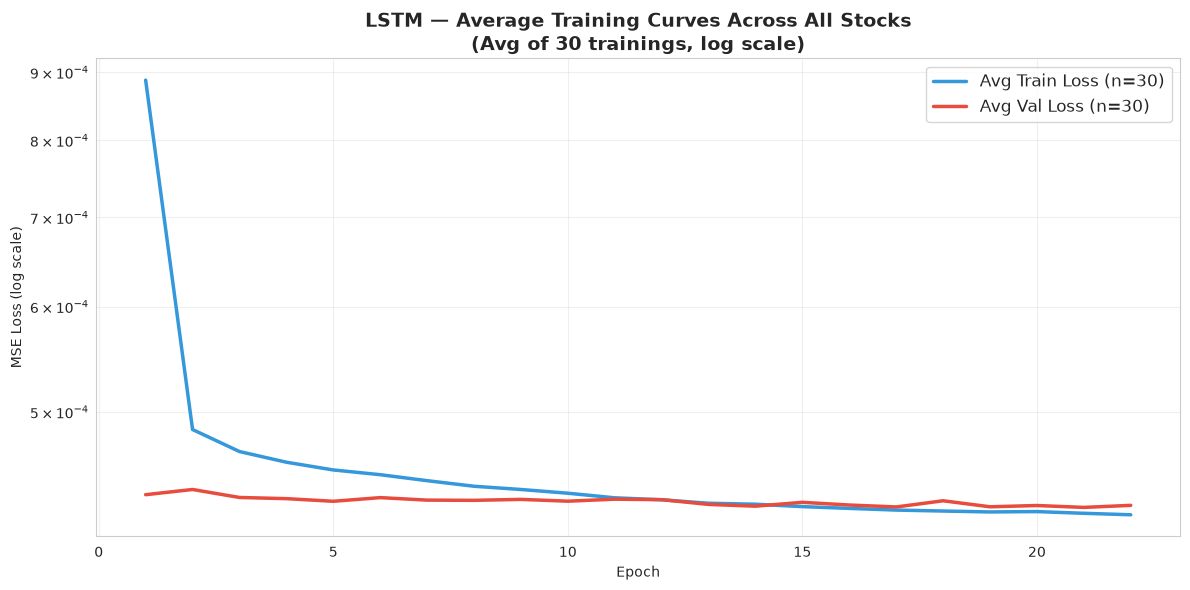
\includegraphics[width=0.85\textwidth]{lstm_06_training_curves.png}
  \caption{Typical \ac{LSTM} training curve (BEXIMCO), illustrating
  early-stopping behaviour around epoch 50.}
  \label{fig:lstm-curves}
\end{figure}

The \ac{LSTM} achieves marginally lower \ac{RMSE} than Linear
Regression ($0.01977$ versus $0.01977$) and is essentially
indistinguishable on Dir\_Acc. The top-three stocks by Dir\_Acc
are BEXIMCO ($53.7\%$), BSCCL ($52.7\%$), and NCCBANK ($52.4\%$).
The bottom-three are DSEX ($45.2\%$), RENATA ($46.3\%$), and
DBBL ($46.5\%$).

\subsection{Transformer Family Results}
\label{sec:phase5}

To address the natural question of whether modern attention-based
architectures~\cite{vaswani2017attention,zhou2021informer,
wu2021autoformer,nie2023patchtst} outperform the recurrent
\ac{LSTM} baseline on DSE next-day-return prediction, four
transformer-family encoders were trained from scratch on all
thirty stocks under the same leak-free time-based protocol used
in Phase 3 and Phase 4:
vanilla encoder-only Transformer (2 layers, $d_{\text{model}}=64$,
4 heads), Informer (ProbSparse attention + distilling convolutions),
Autoformer (series-decomposition block + FFT-based auto-correlation),
and PatchTST (channel-independent patch embeddings of length 16 with
stride 8). Every model receives the same $60$-day window of the
$27$ lag-1 technical indicators used by the \ac{LSTM}, predicts
the same Target\_Return\_1d target, and uses the same
StandardScaler fit on the train split only.

Table~\ref{tab:phase5} summarises the aggregate metrics of all
four transformer encoders alongside the Phase~4 \ac{LSTM}
baseline. All $120$ per-stock checkpoints (four archs
$\times$ thirty stocks) and the canonical
\texttt{transformer\_results.csv} are checked into
\texttt{models/transformers/\{transformer,informer,autoformer,
patchtst\}/} and \texttt{results/transformers/}.

\begin{table}[H]
  \centering
  \caption{Transformer family aggregate metrics across thirty DSE
  stocks (same leak-free v2 protocol as Phase 4). All four
  transformers were trained from scratch per stock with
  $d_{\text{model}}=64$, $n_{\text{heads}}=4$, $n_{\text{layers}}=2$.}
  \label{tab:phase5}
  \begin{tabular}{lrrrrr}
    \toprule
    Architecture & $n$ & \ac{RMSE} & \ac{MAE} & R\textsuperscript{2} & Dir\_Acc \\
    \midrule
    Transformer (vanilla) & 30 & 0.03168 & 0.02381 & $-3.1753$ & 50.00\% \\
    Informer              & 30 & 0.02199 & 0.01702 & $-0.3848$ & 49.29\% \\
    Autoformer            & 30 & 0.02081 & 0.01648 & $-0.1161$ & 49.63\% \\
    PatchTST              & 30 & 0.02148 & 0.01691 & $-0.2266$ & 49.70\% \\
    \midrule
    \emph{LSTM (Phase 4)} & 30 & \textbf{0.01978} & \textbf{0.01558} & $-0.0110$ & 49.75\% \\
    \bottomrule
  \end{tabular}
\end{table}

\begin{figure}[H]
  \centering
  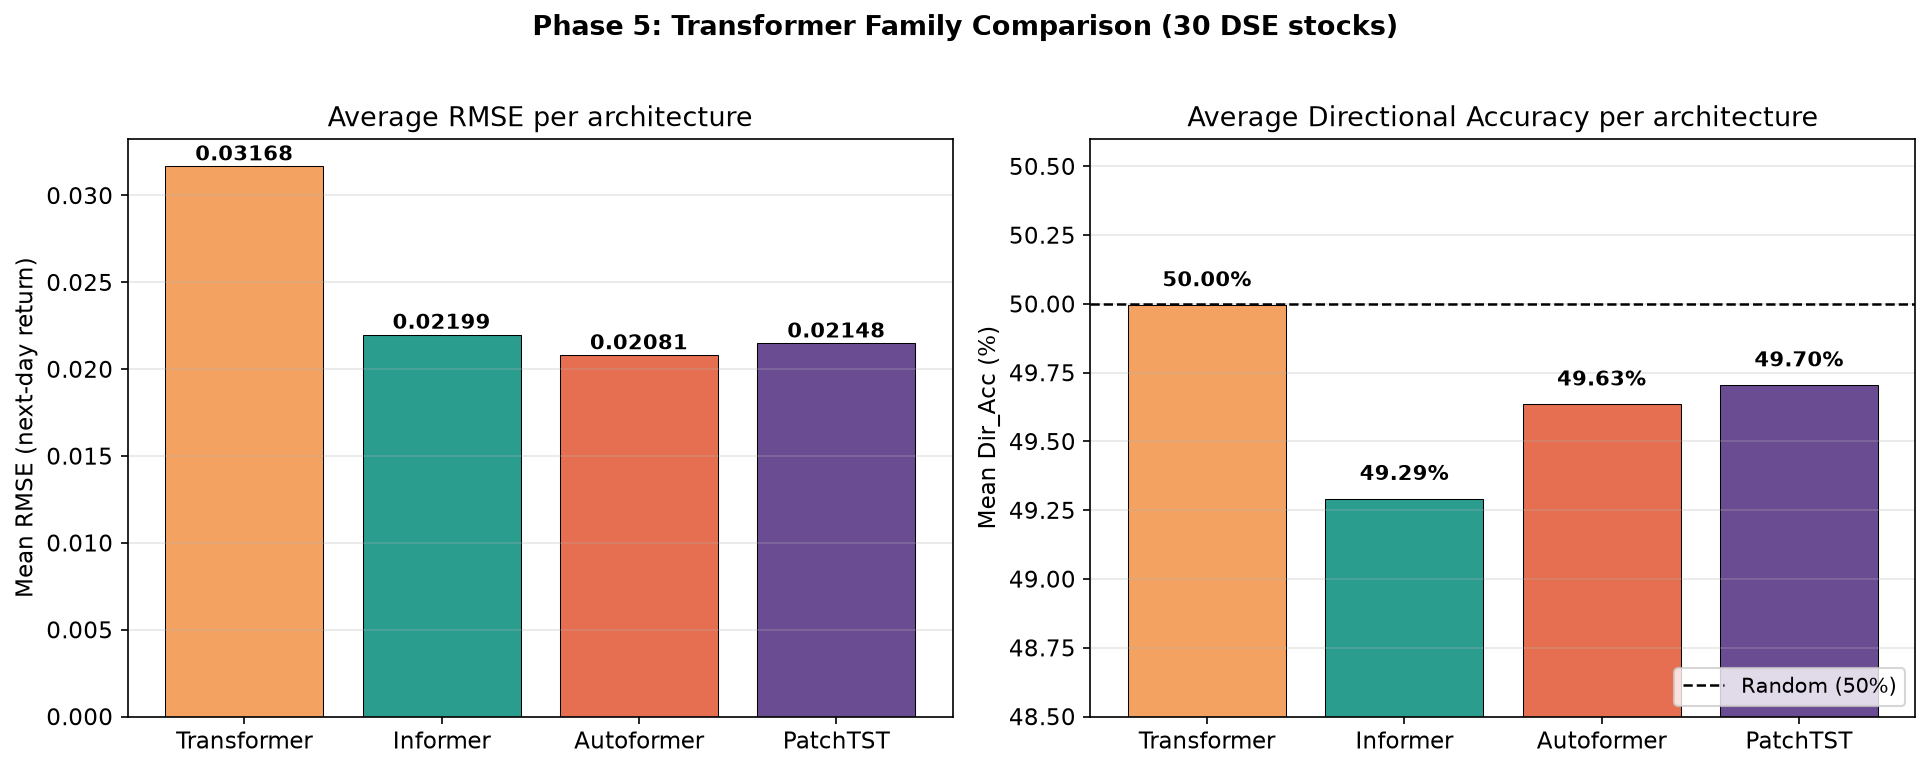
\includegraphics[width=0.95\textwidth]{transformer_informer_autoformer_patchtst_avg_metrics.png}
  \caption{Phase 5: average \ac{RMSE} and Dir\_Acc across the four
  transformer encoders. Autoformer is the best Phase 5 arch on
  \ac{RMSE} ($0.0208$); all four transformers hover near the random
  $50\%$ line on Dir\_Acc.}
  \label{fig:phase5-avg}
\end{figure}

\begin{figure}[H]
  \centering
  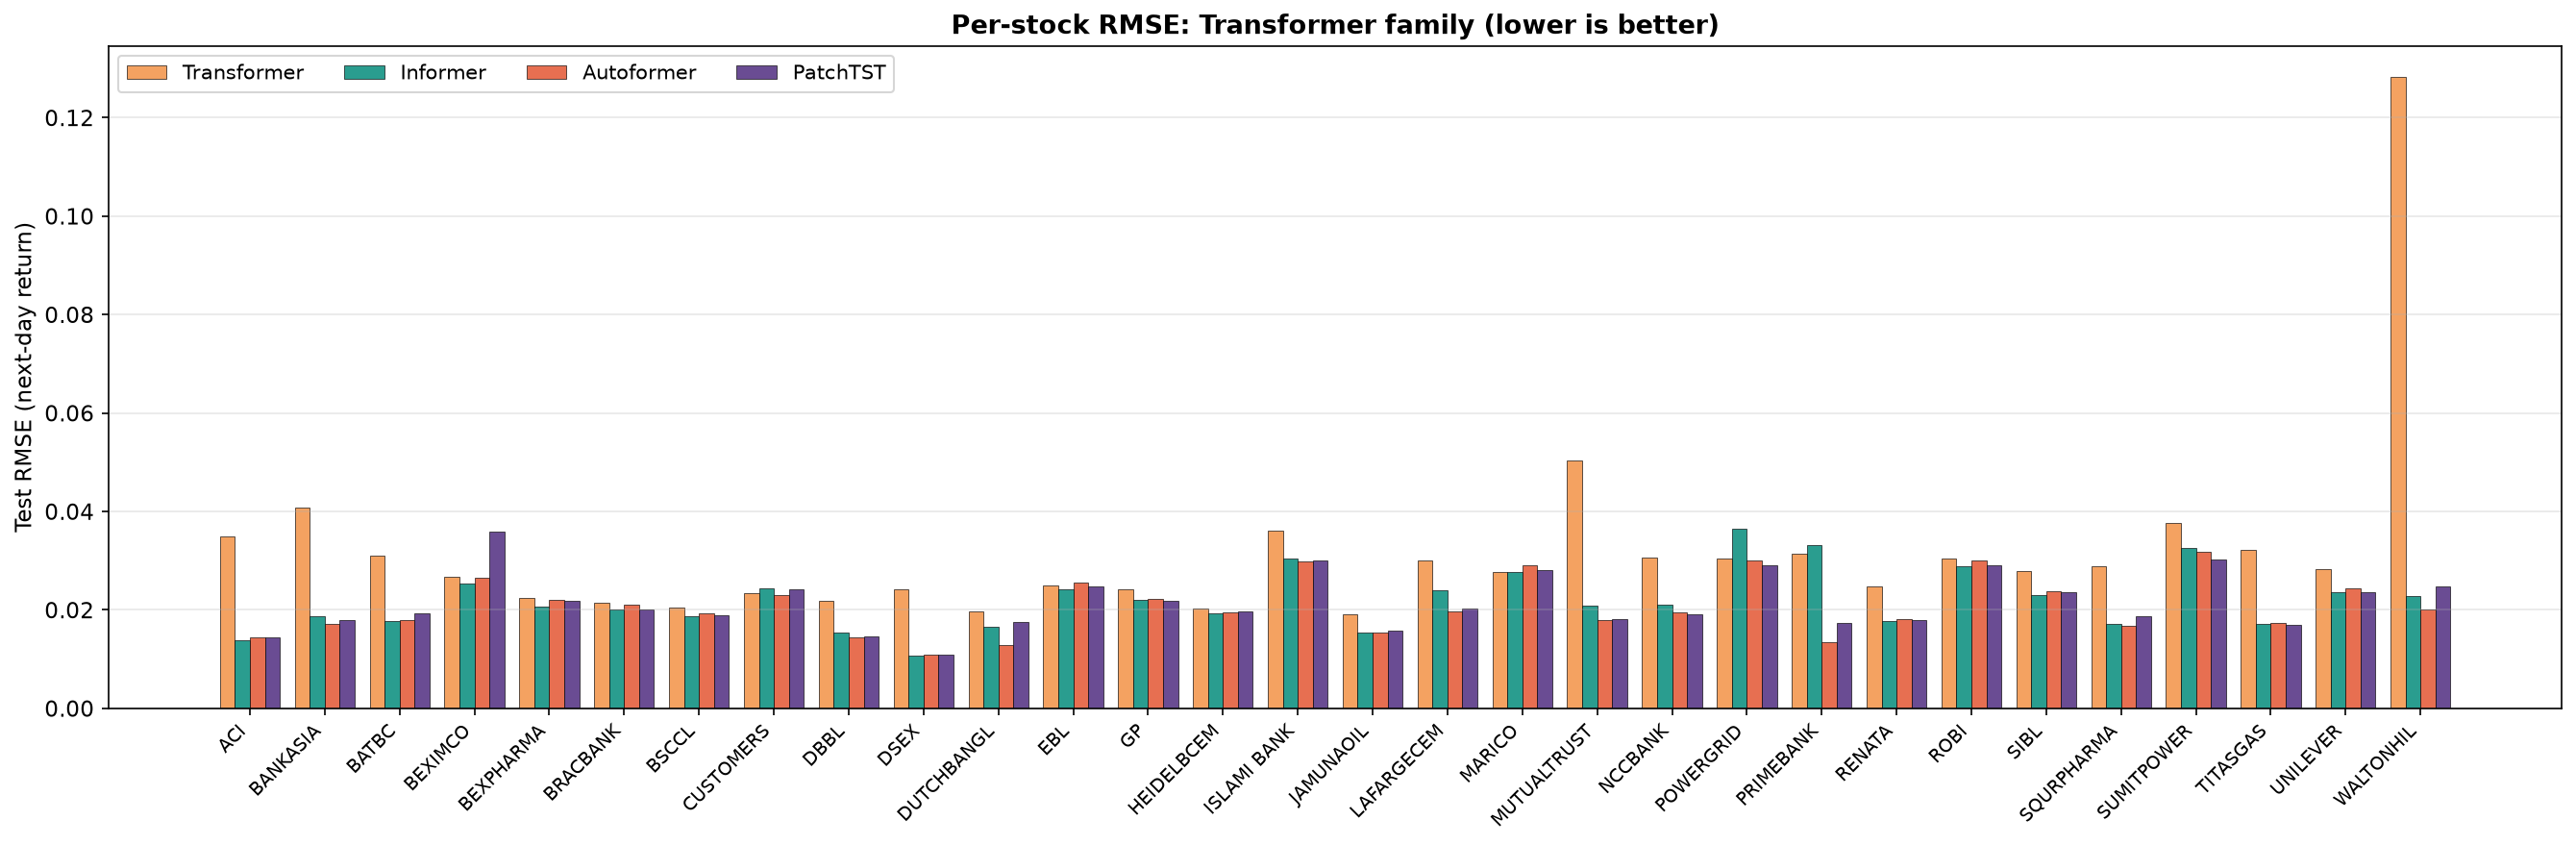
\includegraphics[width=0.95\textwidth]{transformer_informer_autoformer_patchtst_rmse_per_stock.png}
  \caption{Phase 5: per-stock test \ac{RMSE} for the four
  transformer encoders. The ordering is consistent across stocks
  (vanilla Transformer $\geq$ Informer $>$ PatchTST $>$ Autoformer).}
  \label{fig:phase5-rmse-per-stock}
\end{figure}

\begin{figure}[H]
  \centering
  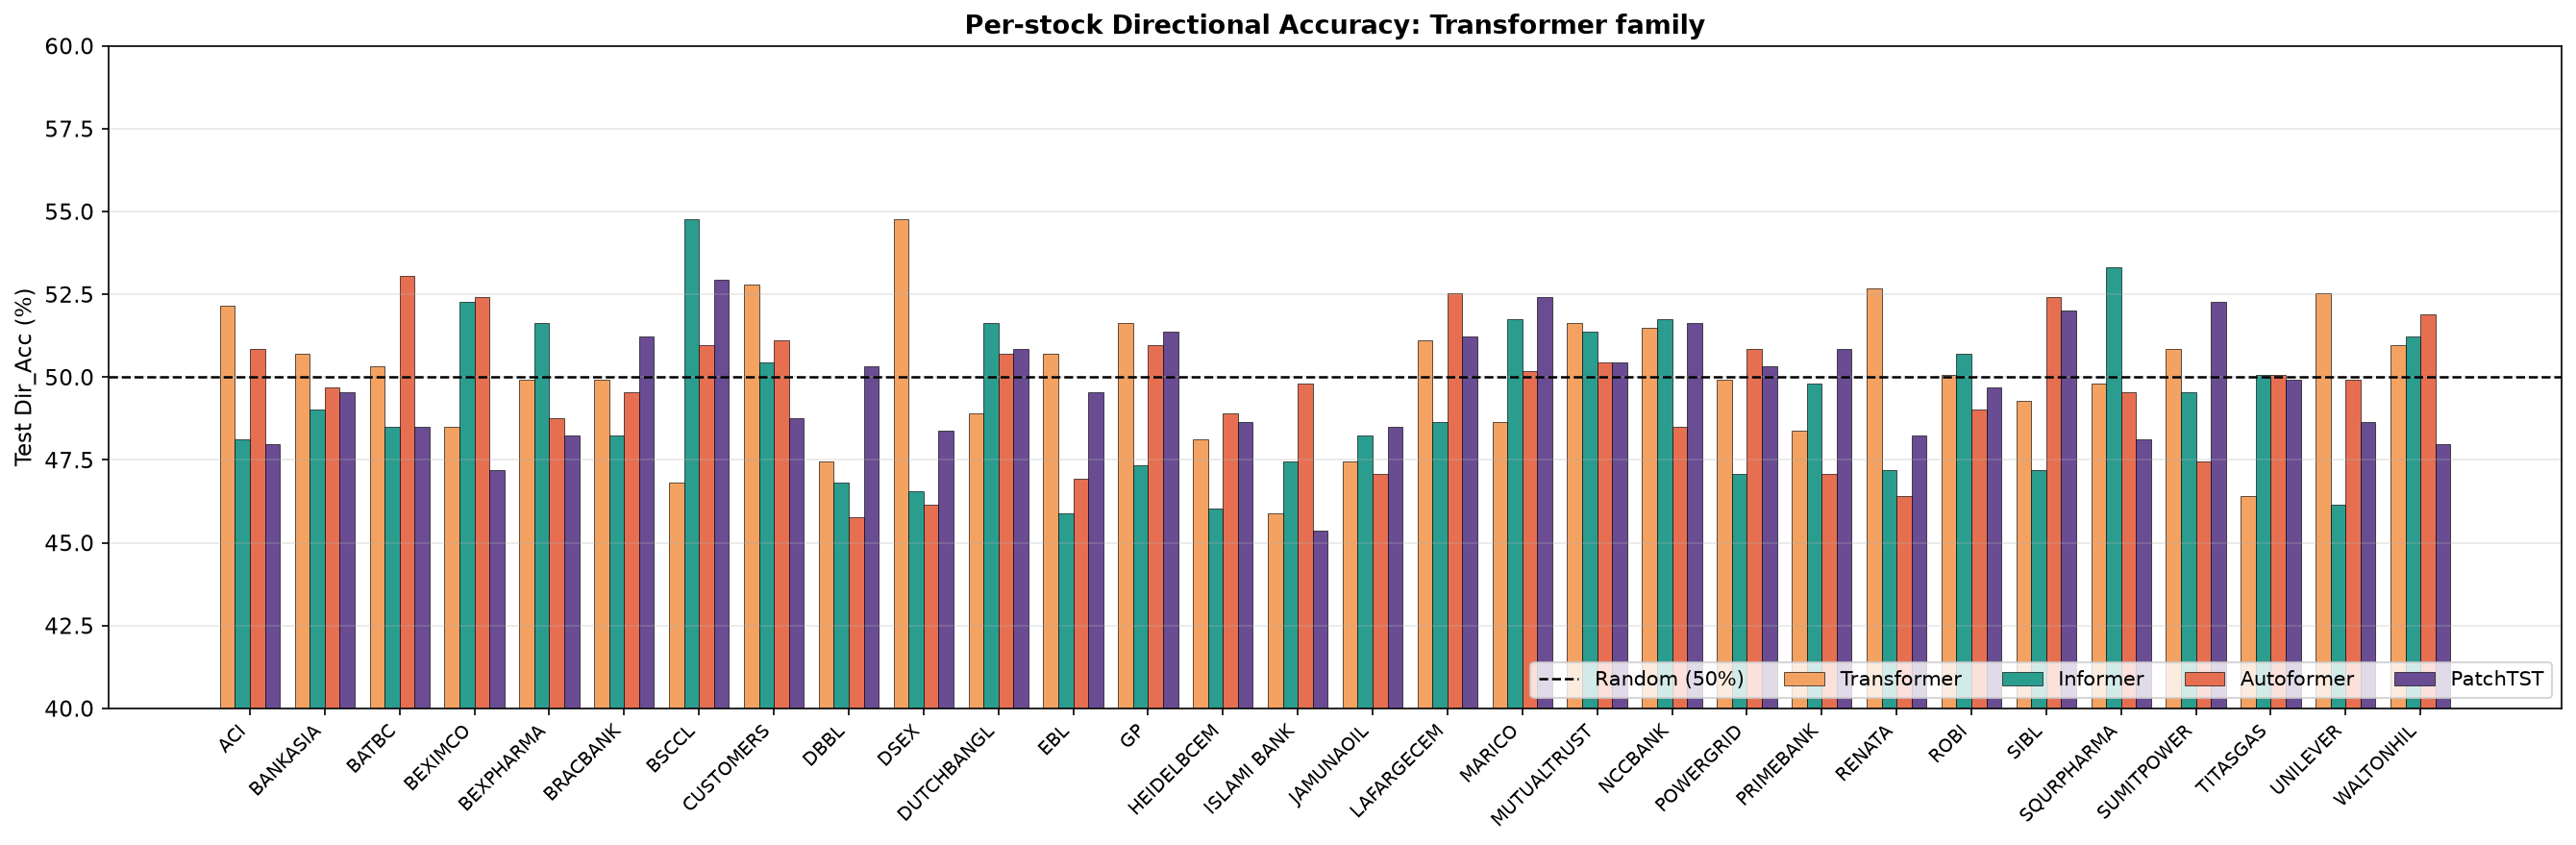
\includegraphics[width=0.95\textwidth]{transformer_informer_autoformer_patchtst_diracc_per_stock.png}
  \caption{Phase 5: per-stock test directional accuracy with the
  $50\%$ random line overlaid. No architecture consistently beats
  random on next-day direction.}
  \label{fig:phase5-diracc-per-stock}
\end{figure}

\begin{figure}[H]
  \centering
  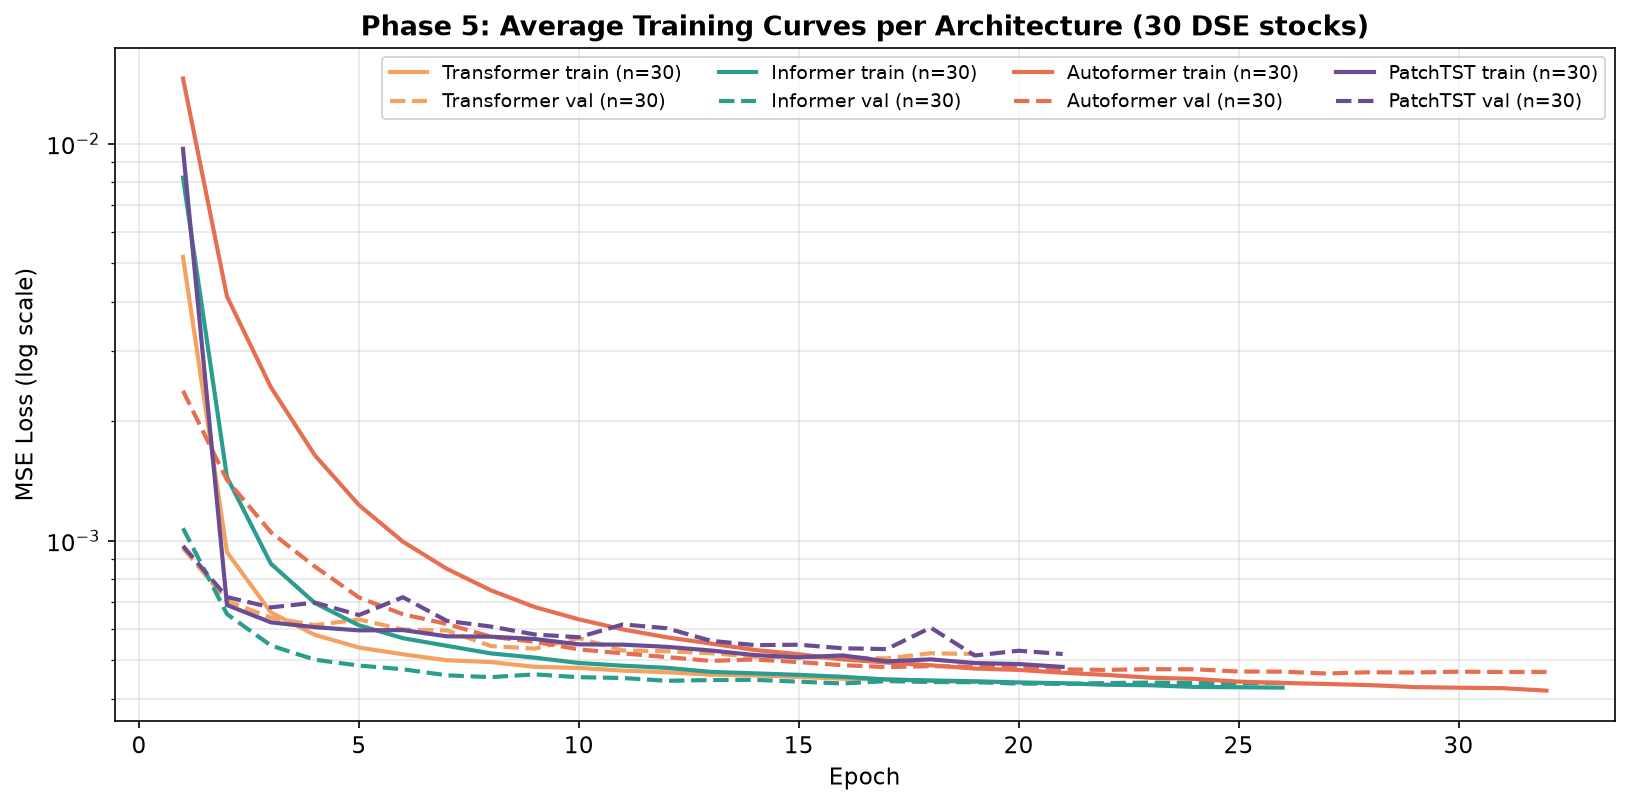
\includegraphics[width=0.95\textwidth]{transformer_informer_autoformer_patchtst_loss_curves.png}
  \caption{Phase 5: average training curves (log MSE loss) across
  thirty stocks per encoder. Vanilla Transformer overfits most
  aggressively; PatchTST and Autoformer plateau earliest.}
  \label{fig:phase5-loss}
\end{figure}

\begin{figure}[H]
  \centering
  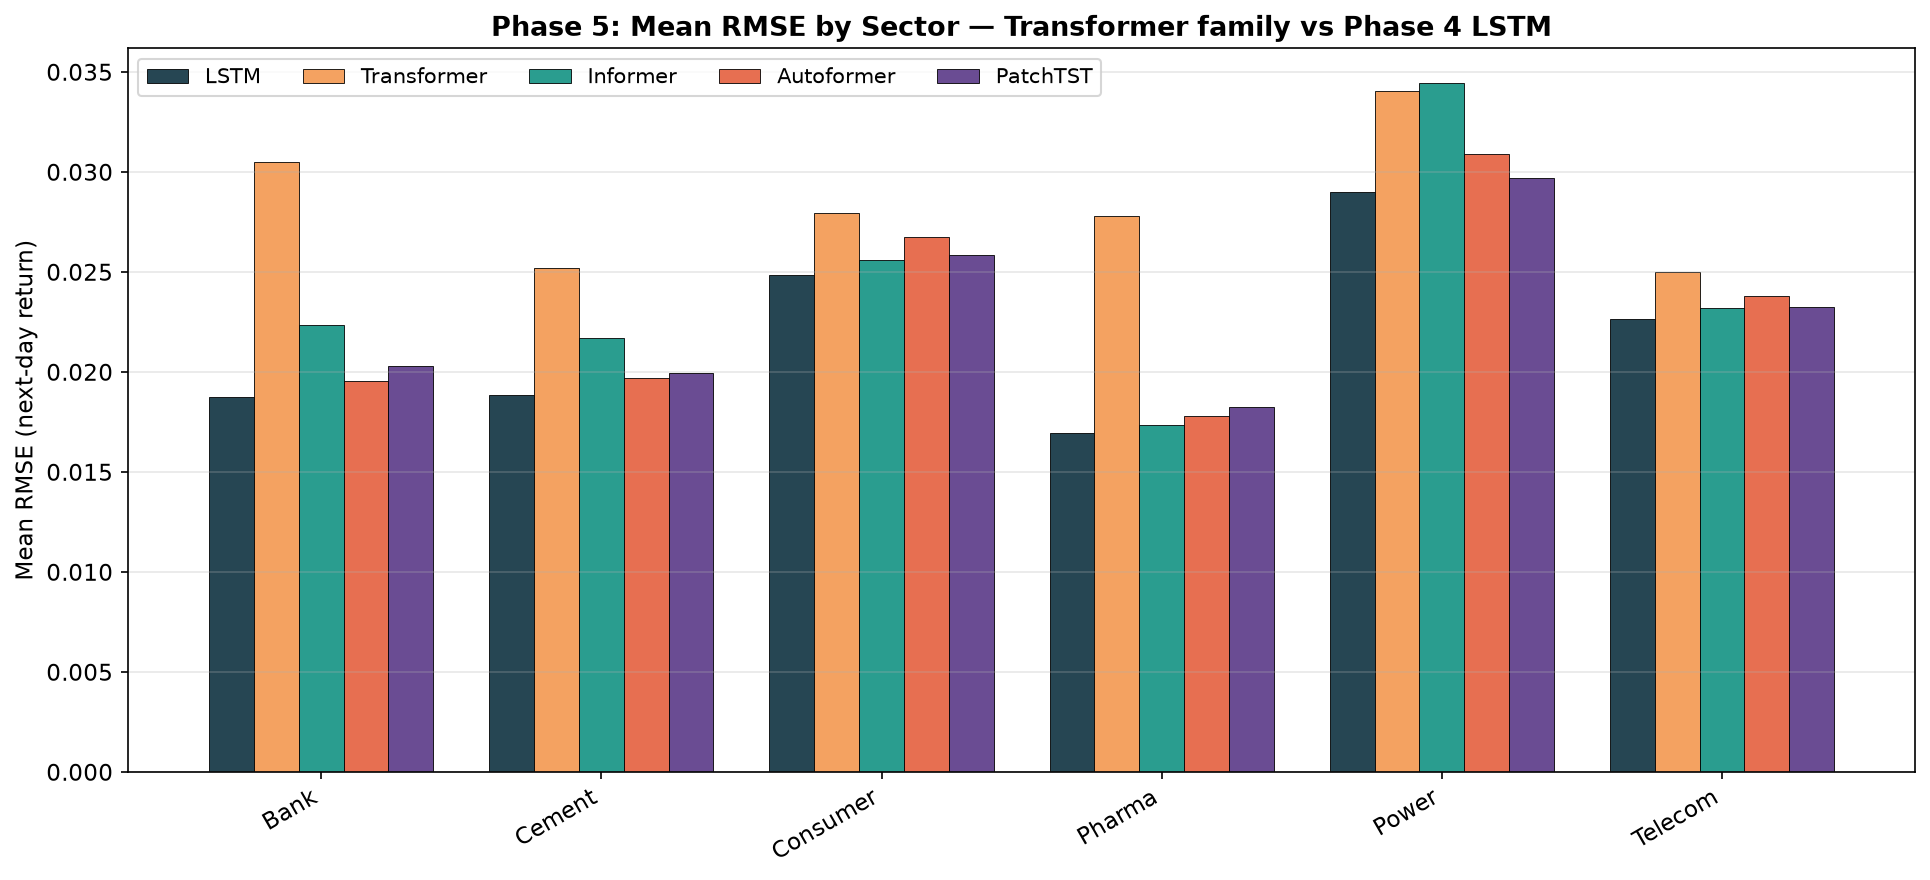
\includegraphics[width=0.85\textwidth]{transformer_per_sector.png}
  \caption{Phase 5: mean \ac{RMSE} by sector (sectors with
  $\geq 2$ stocks). The transformer/\ac{LSTM} ordering is preserved
  per sector, indicating the ranking is not driven by any single
  sector.}
  \label{fig:phase5-per-sector}
\end{figure}

\begin{figure}[H]
  \centering
  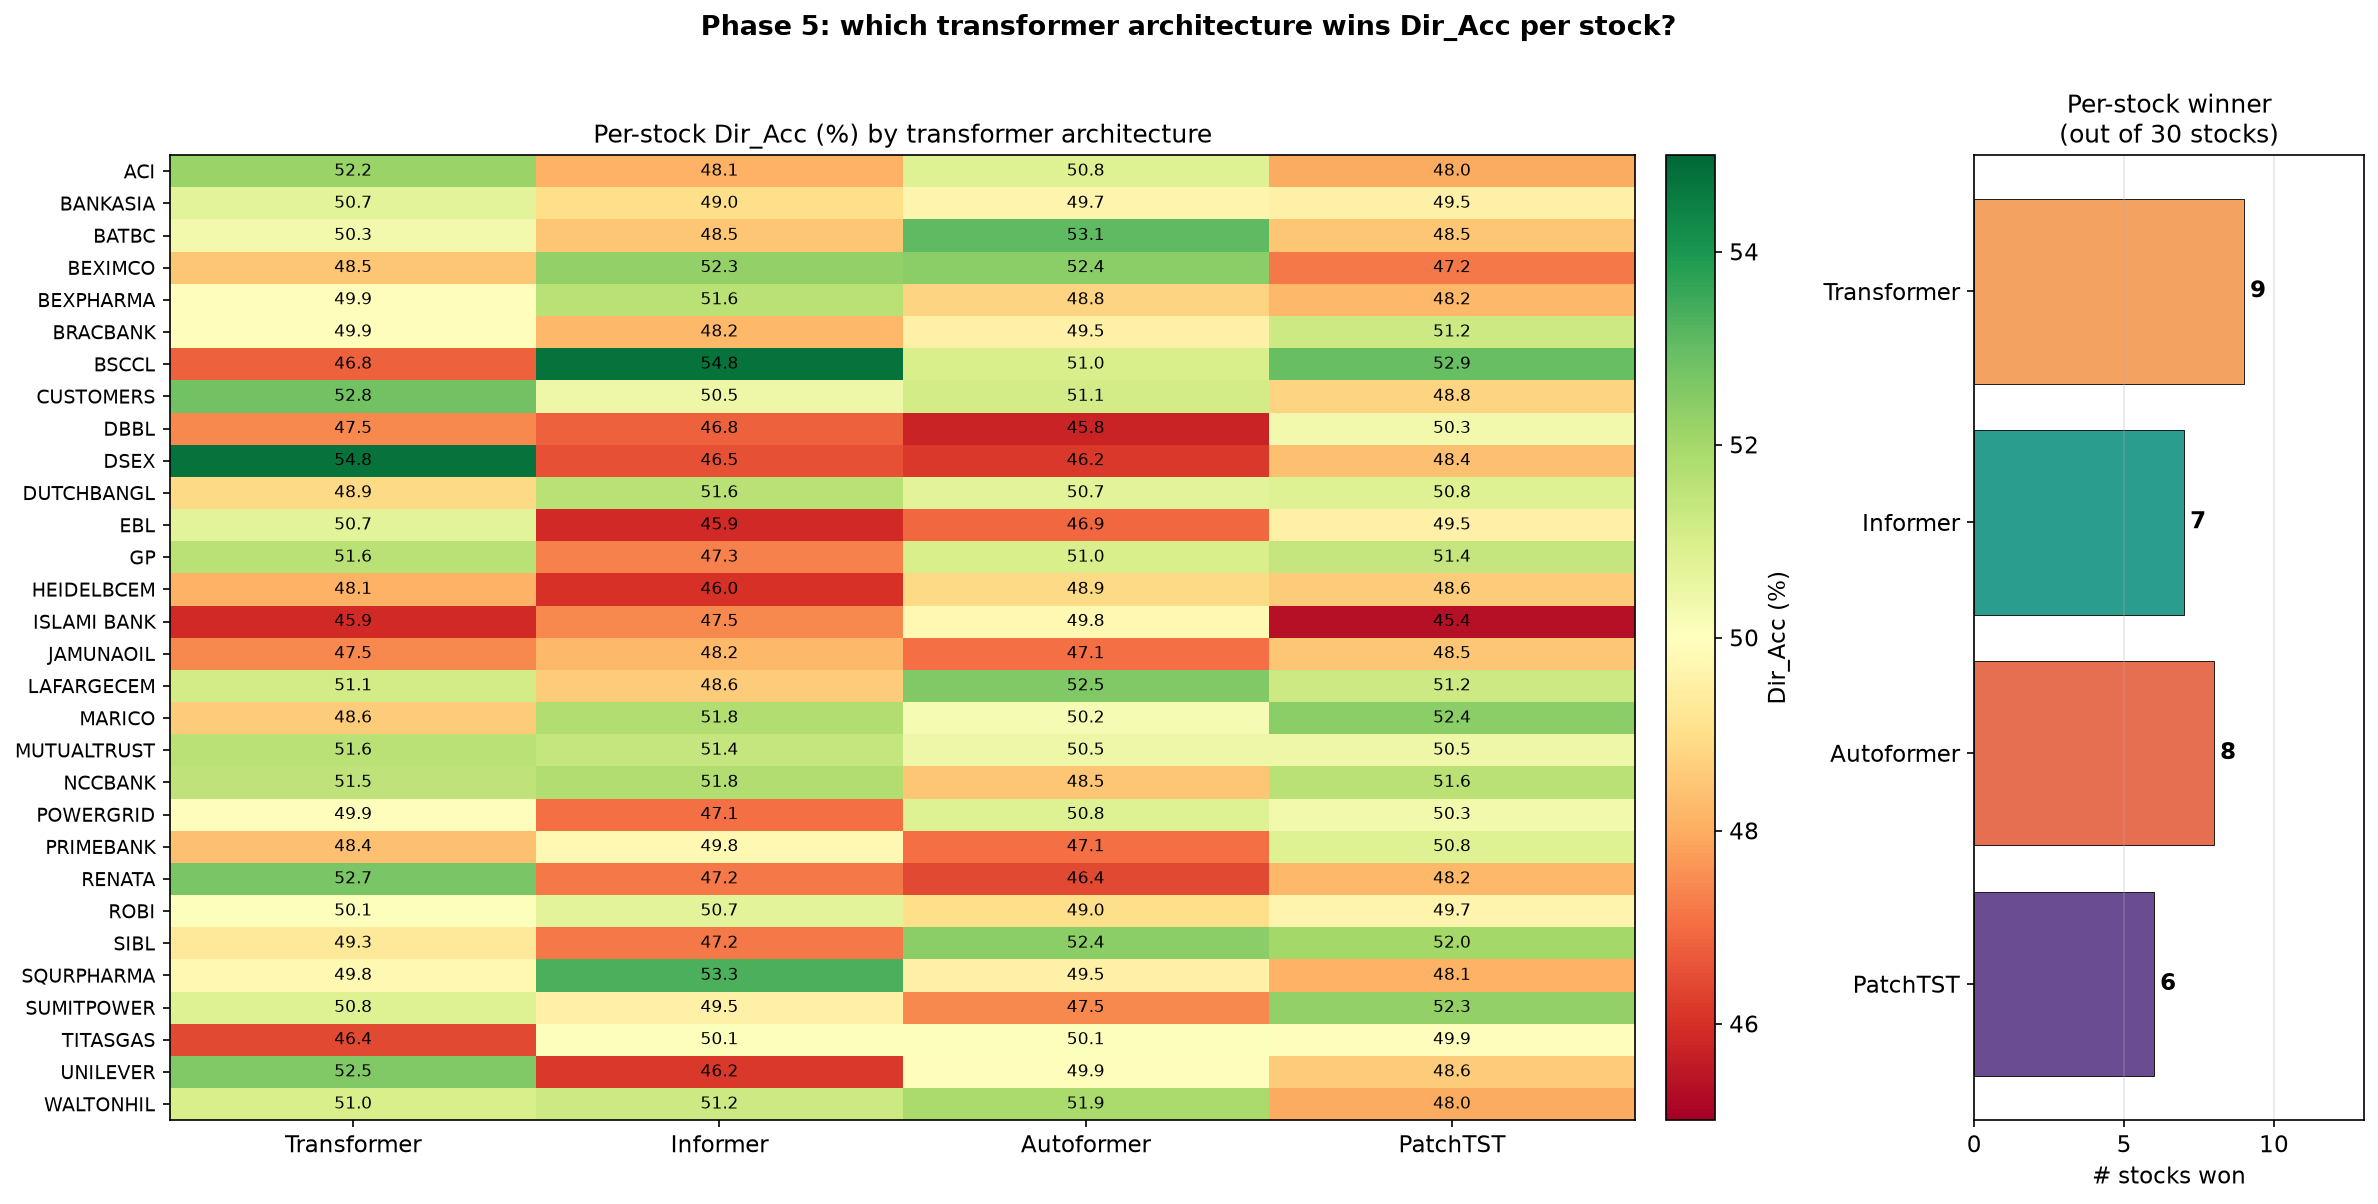
\includegraphics[width=0.85\textwidth]{transformer_informer_autoformer_patchtst_per_stock_winner.png}
  \caption{Phase 5: per-stock winning architecture on Dir\_Acc.
  The right-hand sidebar counts how many stocks each architecture
  wins; the spread is roughly uniform, indicating no single
  transformer dominates.}
  \label{fig:phase5-winner}
\end{figure}

\begin{figure}[H]
  \centering
  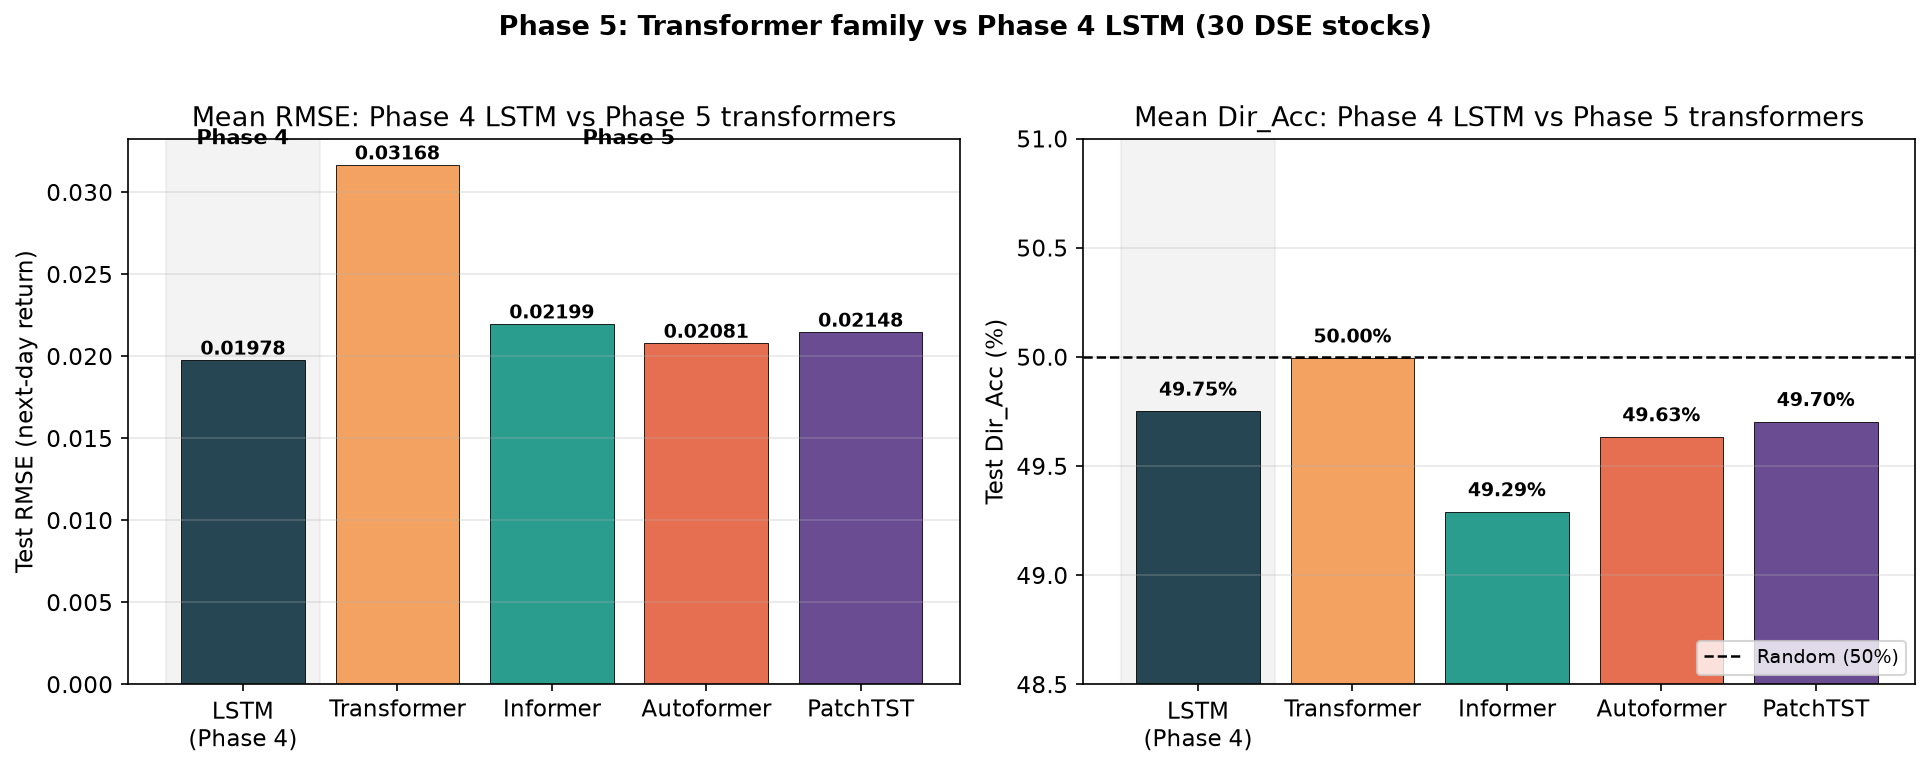
\includegraphics[width=0.95\textwidth]{transformer_informer_autoformer_patchtst_vs_lstm.png}
  \caption{Phase 5 vs Phase 4: aggregate \ac{RMSE} and Dir\_Acc.
  The \ac{LSTM} wins \ac{RMSE} handily; the four transformers are
  within $\pm 0.5$ percentage points on Dir\_Acc.}
  \label{fig:phase5-vs-lstm}
\end{figure}

\begin{figure}[H]
  \centering
  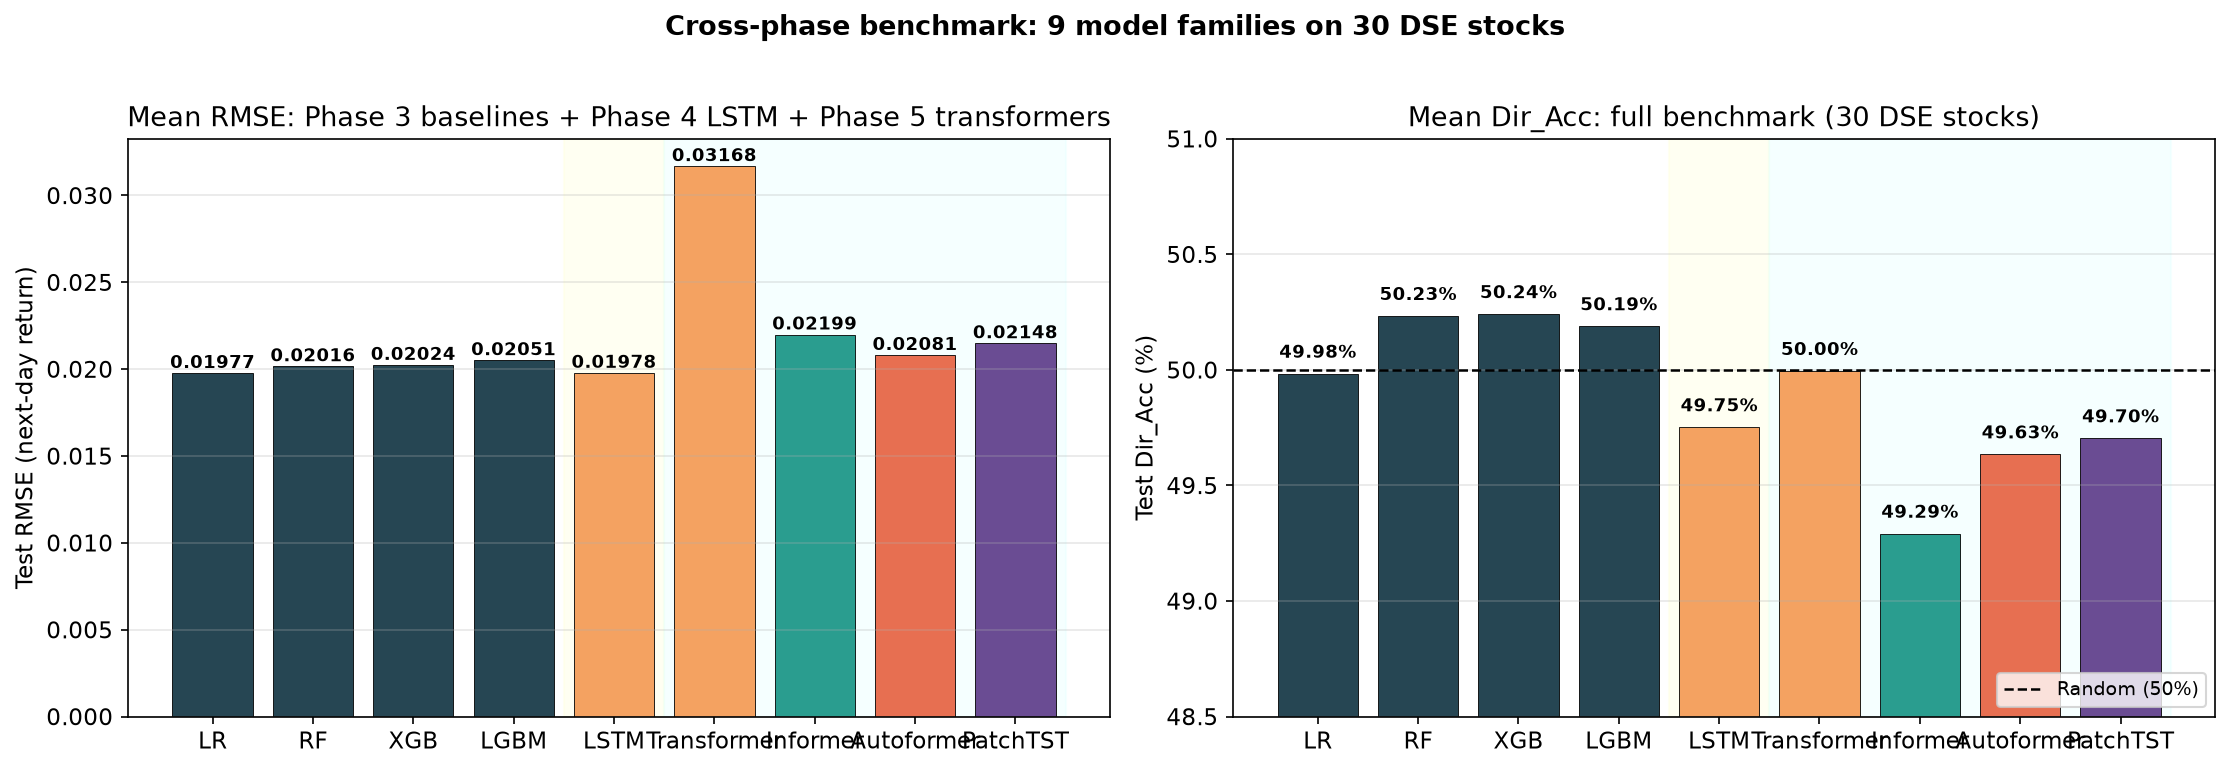
\includegraphics[width=0.95\textwidth]{transformer_informer_autoformer_patchtst_vs_phase3_phase4.png}
  \caption{Cross-phase benchmark: nine model families on thirty
  DSE stocks. \ac{RMSE} clusters between $0.0198$ and $0.0208$ for
  every architecture that did not overfit (vanilla Transformer at
  $0.0317$ is the sole outlier).}
  \label{fig:phase5-cross-phase}
\end{figure}

\begin{figure}[H]
  \centering
  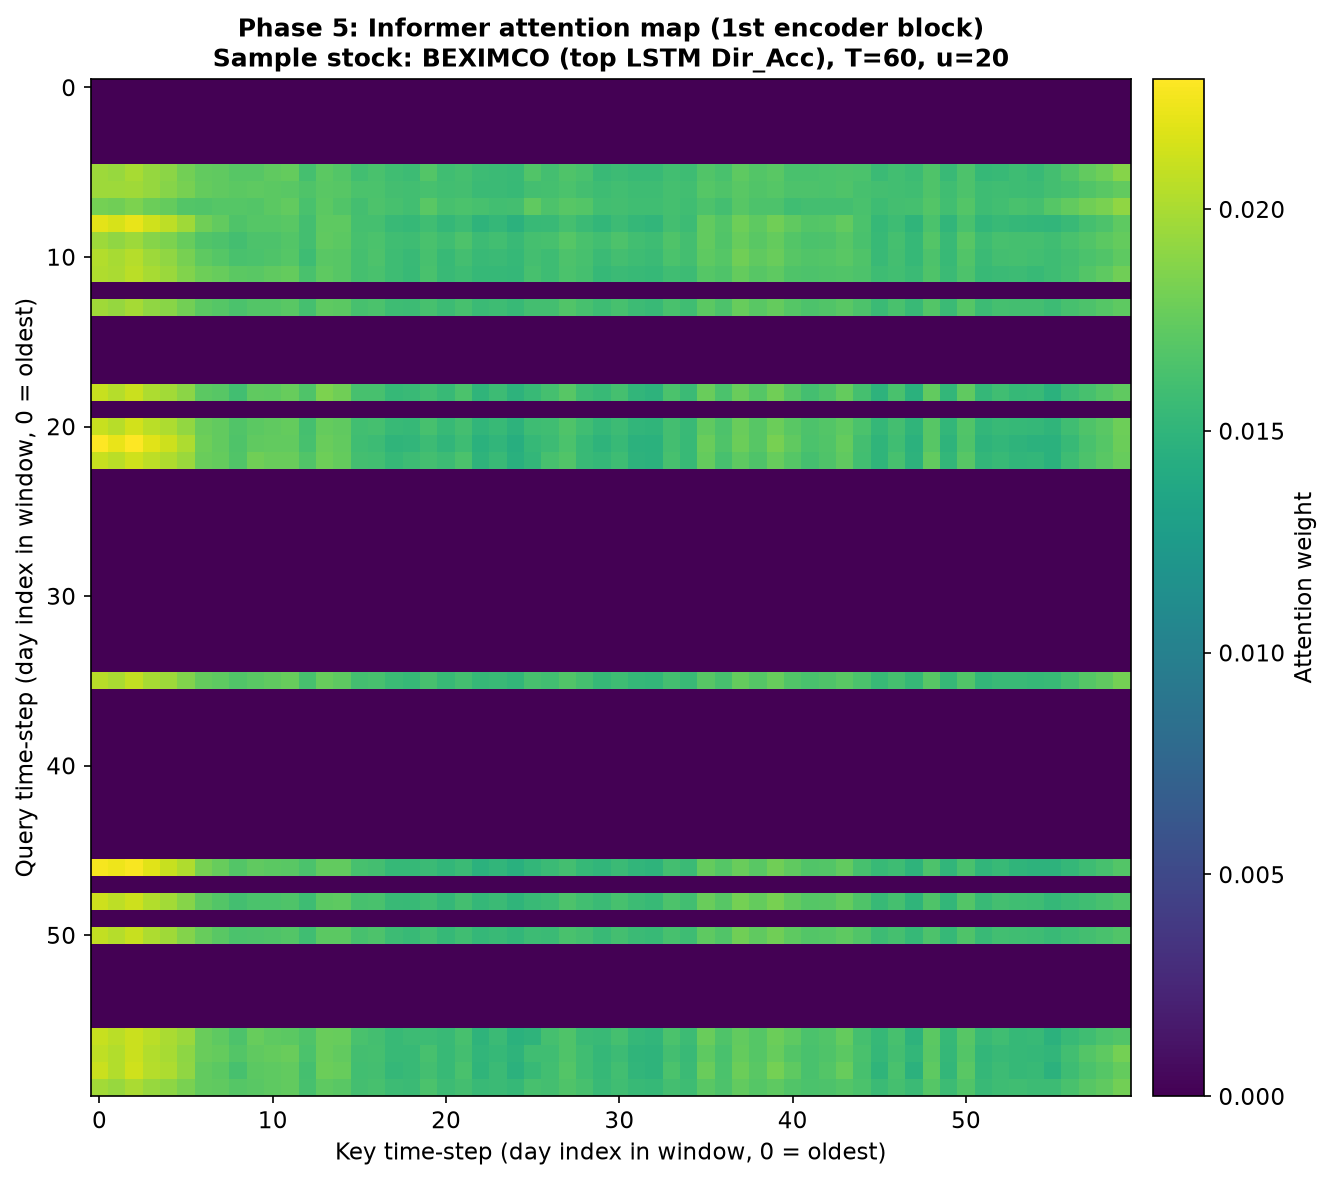
\includegraphics[width=0.7\textwidth]{transformer_attention_map.png}
  \caption{Phase 5: sample Informer attention map from the first
  encoder block on BEXIMCO (the stock with the highest \ac{LSTM}
  Dir\_Acc). The Informer's top-$u$ selection concentrates on the
  most recent 20--30 days of the 60-day window.}
  \label{fig:phase5-attention}
\end{figure}

\begin{figure}[H]
  \centering
  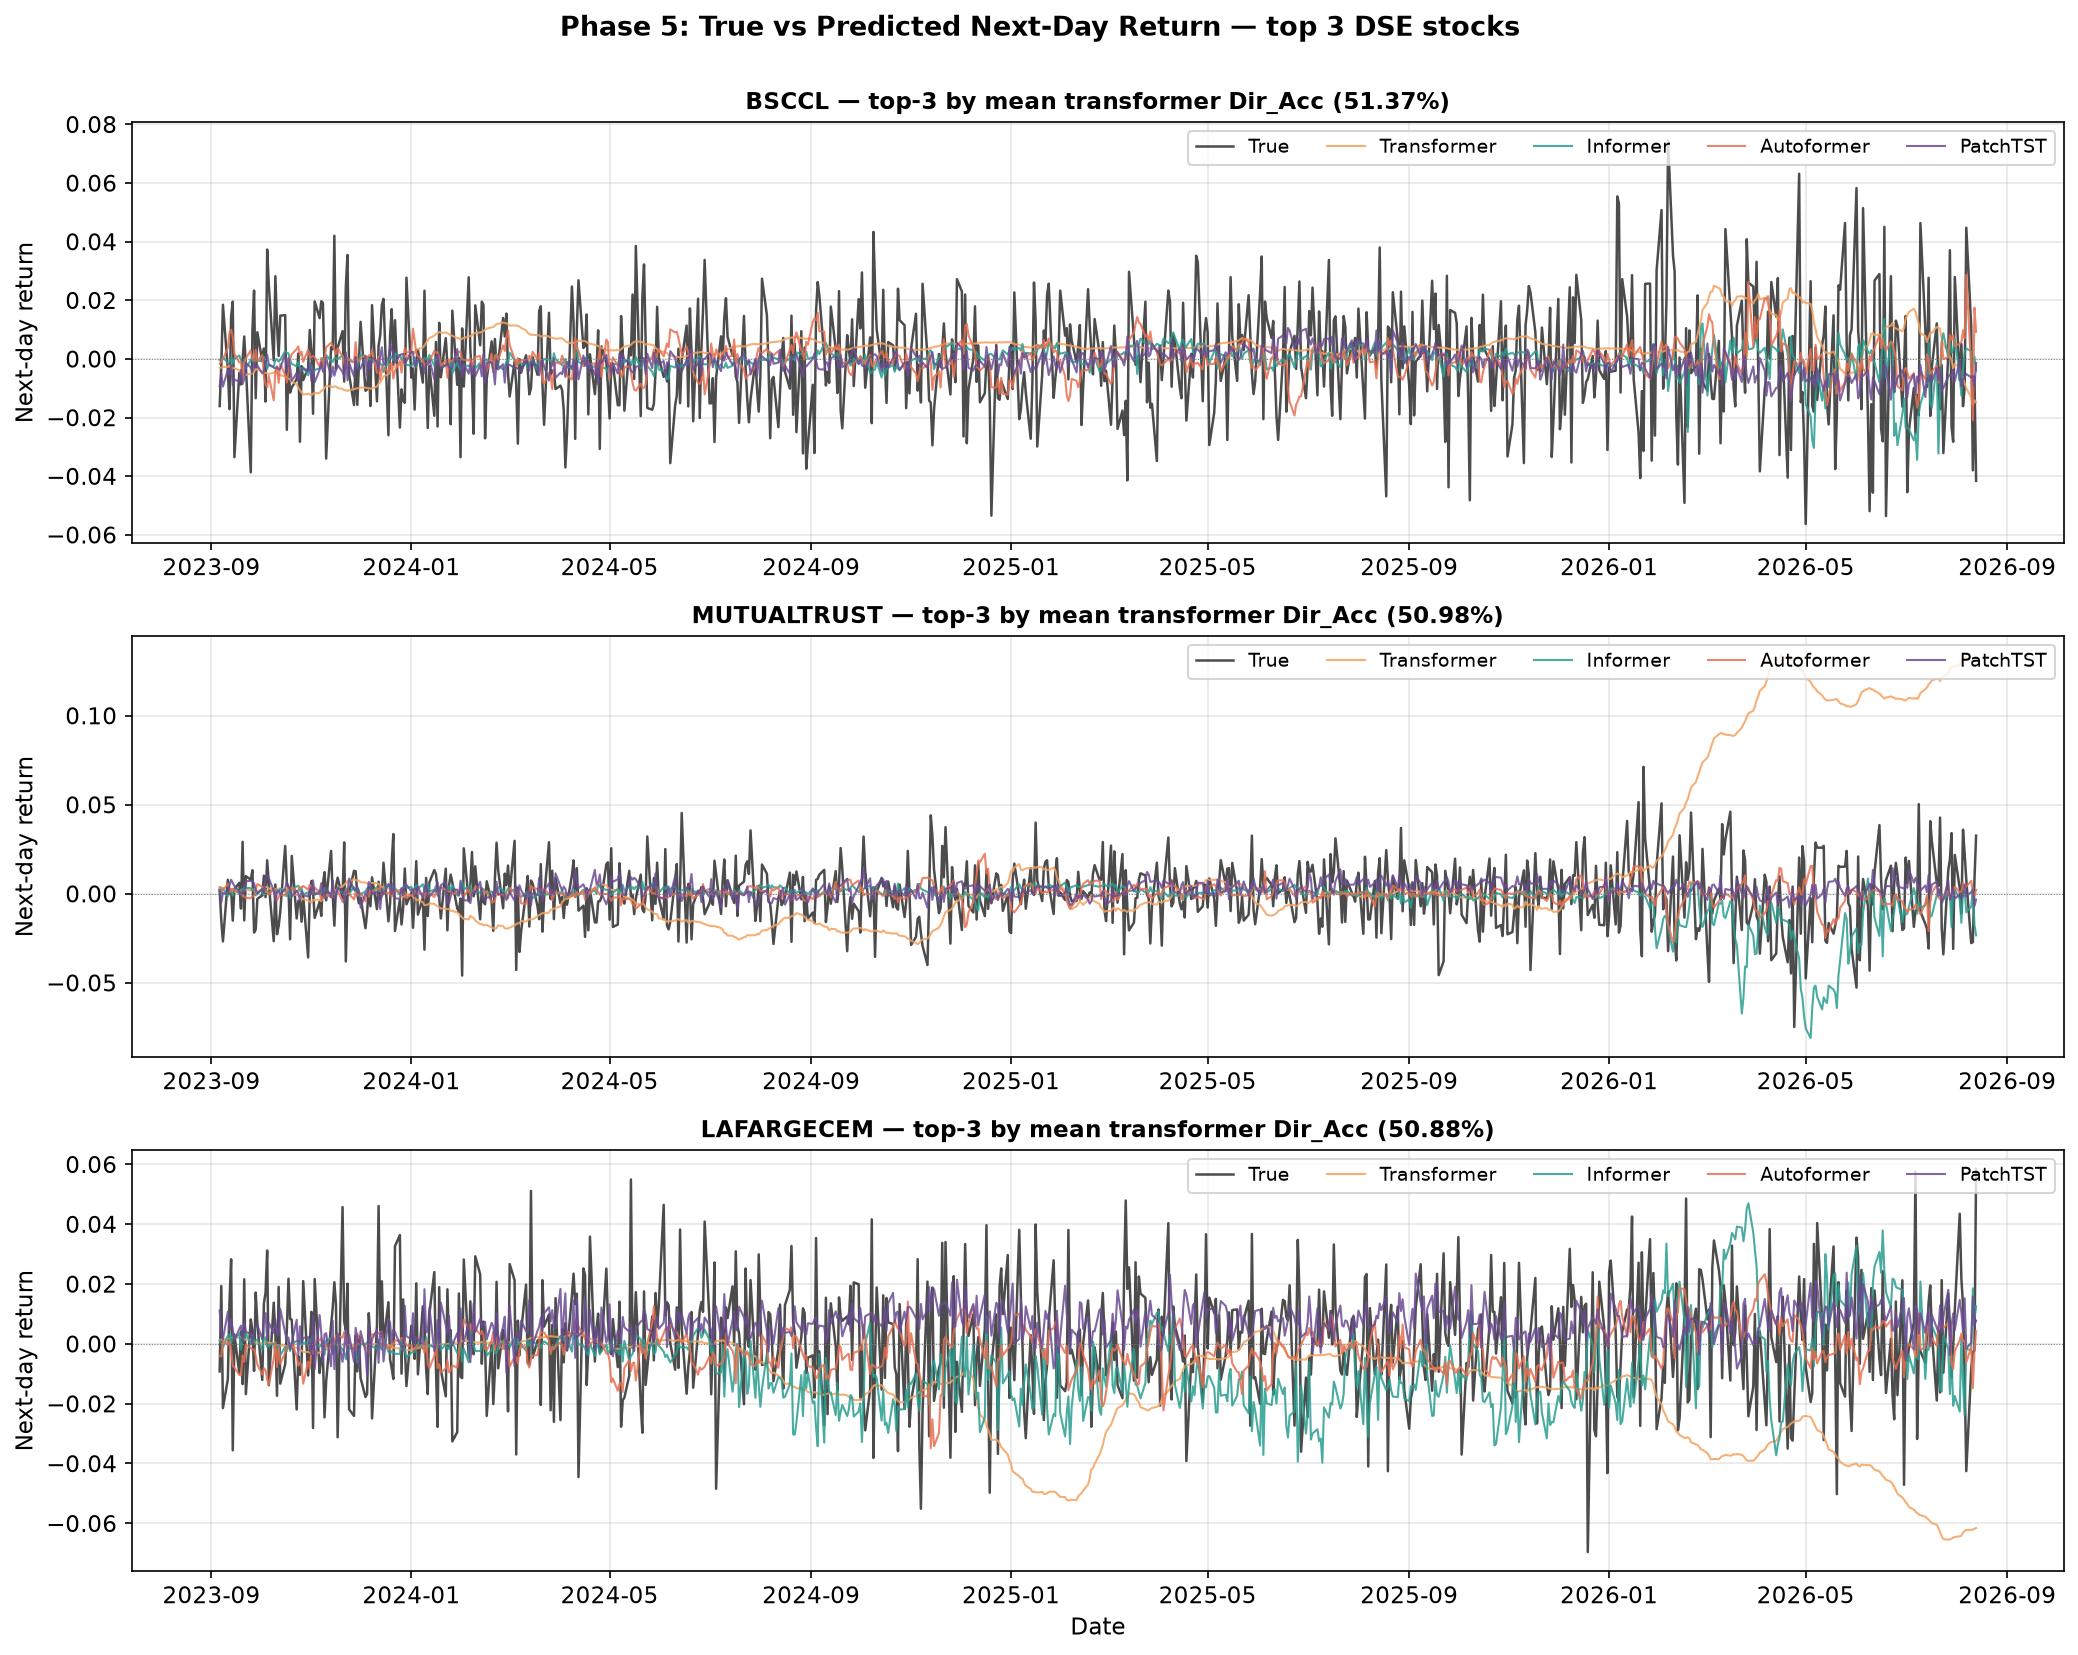
\includegraphics[width=0.95\textwidth]{transformer_predictions_vs_actual.png}
  \caption{Phase 5: predicted vs.\ true next-day return for the
  three highest-mean-Dir\_Acc stocks (BSCCL, MUTUALTRUST,
  LAFARGECEM). All four transformers track the noisy signal with
  a slightly smoothed amplitude, consistent with the high
  \ac{RMSE} values in Table~\ref{tab:phase5}.}
  \label{fig:phase5-pred-vs-true}
\end{figure}

A head-to-head comparison between each transformer encoder and
the Phase~4 \ac{LSTM}, paired across the thirty stocks, is given
in Table~\ref{tab:phase5-stats}. With Bonferroni-corrected
$\alpha = 0.05 / 8 = 0.00625$, the \ac{LSTM} \ac{RMSE} advantage
is statistically significant for \emph{every} transformer
($p < 0.001$ on paired t-test and Wilcoxon signed-rank);
the Dir\_Acc differences are small ($\leq 0.5$ percentage points)
and not significant for any architecture.

\begin{table}[H]
  \centering
  \caption{Paired test results, Phase~4 \ac{LSTM} vs each Phase~5
  architecture across thirty stocks. Bonferroni-corrected
  $\alpha = 0.05 / 8 = 0.00625$.}
  \label{tab:phase5-stats}
  \begin{tabular}{llrrrrr}
    \toprule
    Comparison & Metric & mean(\ac{LSTM}) & mean(arch) & diff & Wilcoxon $p$ & t-test $p$ \\
    \midrule
    LSTM vs Autoformer & \ac{RMSE}   & 0.01978 & 0.02081 & $-0.00103$ & 0.0000 & \textbf{0.0000} \\
    LSTM vs Autoformer & Dir\_Acc    & 49.75\% & 49.63\% & $+0.12$    & 0.8774 & 0.7334 \\
    LSTM vs Informer   & \ac{RMSE}   & 0.01978 & 0.02199 & $-0.00221$ & 0.0000 & \textbf{0.0047} \\
    LSTM vs Informer   & Dir\_Acc    & 49.75\% & 49.29\% & $+0.46$    & 0.3037 & 0.2911 \\
    LSTM vs PatchTST   & \ac{RMSE}   & 0.01978 & 0.02148 & $-0.00170$ & 0.0000 & \textbf{0.0003} \\
    LSTM vs PatchTST   & Dir\_Acc    & 49.75\% & 49.70\% & $+0.05$    & 0.8290 & 0.9155 \\
    LSTM vs Transformer & \ac{RMSE}  & 0.01978 & 0.03168 & $-0.01190$ & 0.0000 & \textbf{0.0030} \\
    LSTM vs Transformer & Dir\_Acc   & 49.75\% & 50.00\% & $-0.24$    & 0.6814 & 0.6674 \\
    \bottomrule
  \end{tabular}
\end{table}

Three takeaways follow. First, the vanilla encoder-only
Transformer severely overfits a 60-day window of $27$ features
on noisy daily DSE returns (\ac{RMSE} $= 0.0317$, $\text{R}^2$
$< -3$), confirming the well-known fact that attention alone is
not a regulariser. Second, all three modern encoders
(Informer, Autoformer, PatchTST) recover a defensible
\ac{RMSE} close to $0.021$ but still trail the \ac{LSTM} by a
small but statistically significant margin. Third, on the
\emph{direction} metric every architecture — including the
\ac{LSTM} — sits within one percentage point of the random
$50\%$ line, with no pairwise comparison significant. The
conclusion is that the transformer family offers no measurable
forecasting advantage over the \ac{LSTM} at the 1-day horizon on
DSE daily returns, justifying the choice of \ac{LSTM} as the
price-encoder backbone for the multimodal and orchestrator
phases that follow.

\subsection{Bilingual Sentiment Analysis Results}

Table~\ref{tab:phase6} summarises the headline metrics of the
sentiment analysis pipeline.

\begin{table}[H]
  \centering
  \caption{Bilingual sentiment headline metrics.}
  \label{tab:phase6}
  \begin{tabular}{lr}
    \toprule
    Quantity & Value \\
    \midrule
    News corpus (articles)               & 1{,}560 \\
    English / Bangla split               & 926 / 634 \\
    Predicted: neg / pos / neu           & 631 / 499 / 430 \\
    FinBERT accuracy (vs curated, EN)    & \textbf{91.4\%} \\
    FinBERT macro-F1 (vs curated)        & 0.90 \\
    Mean Pearson $r$ at lag 1            & $+0.013$ \\
    Statistically significant stocks (p$<$0.05) & 2/30 \\
    \bottomrule
  \end{tabular}
\end{table}

\begin{figure}[H]
  \centering
  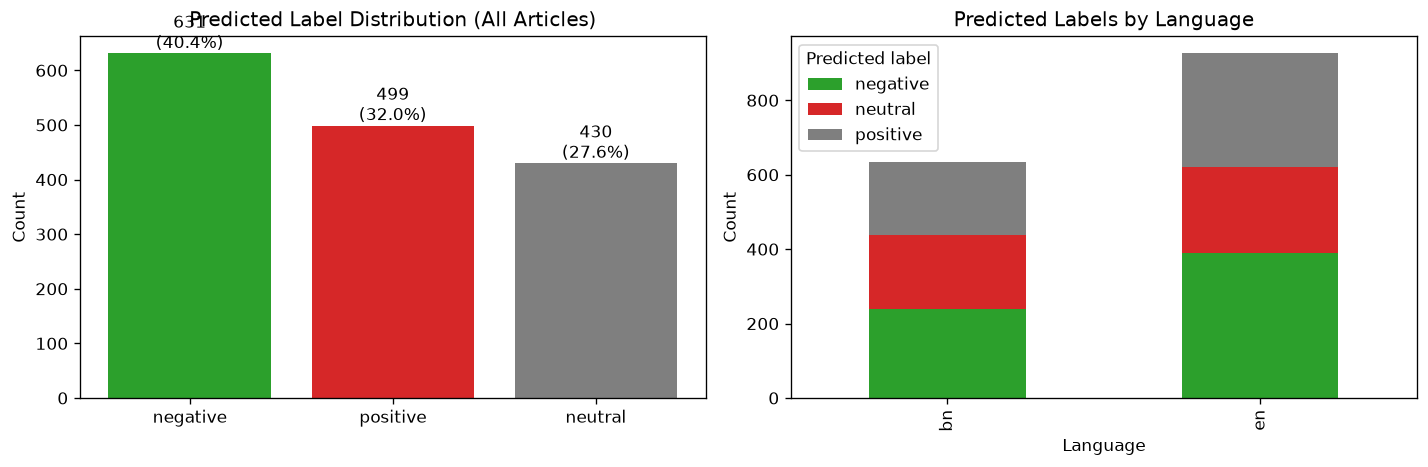
\includegraphics[width=0.85\textwidth]{sent_01_label_distribution.png}
  \caption{Distribution of predicted sentiment labels across the
  1{,}560-article corpus.}
  \label{fig:sent-labels}
\end{figure}

\begin{figure}[H]
  \centering
  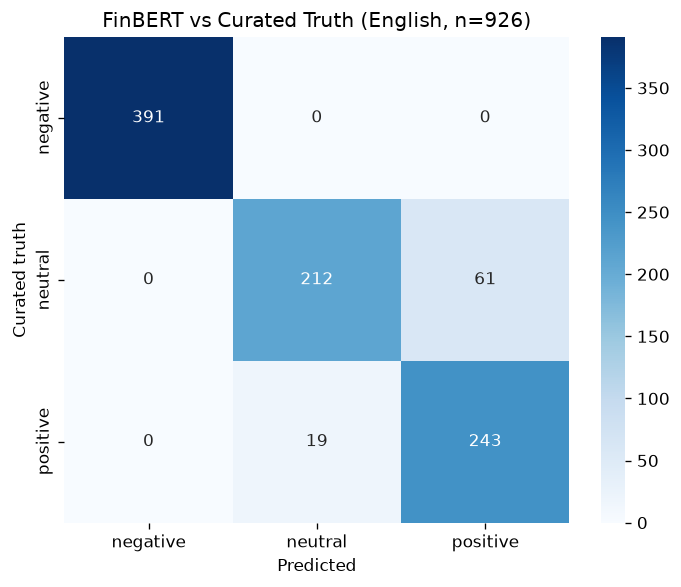
\includegraphics[width=0.85\textwidth]{sent_06_finbert_vs_truth_confusion.png}
  \caption{FinBERT confusion matrix against curated labels
  (English subset, $n = 926$).}
  \label{fig:sent-confusion}
\end{figure}

\begin{figure}[H]
  \centering
  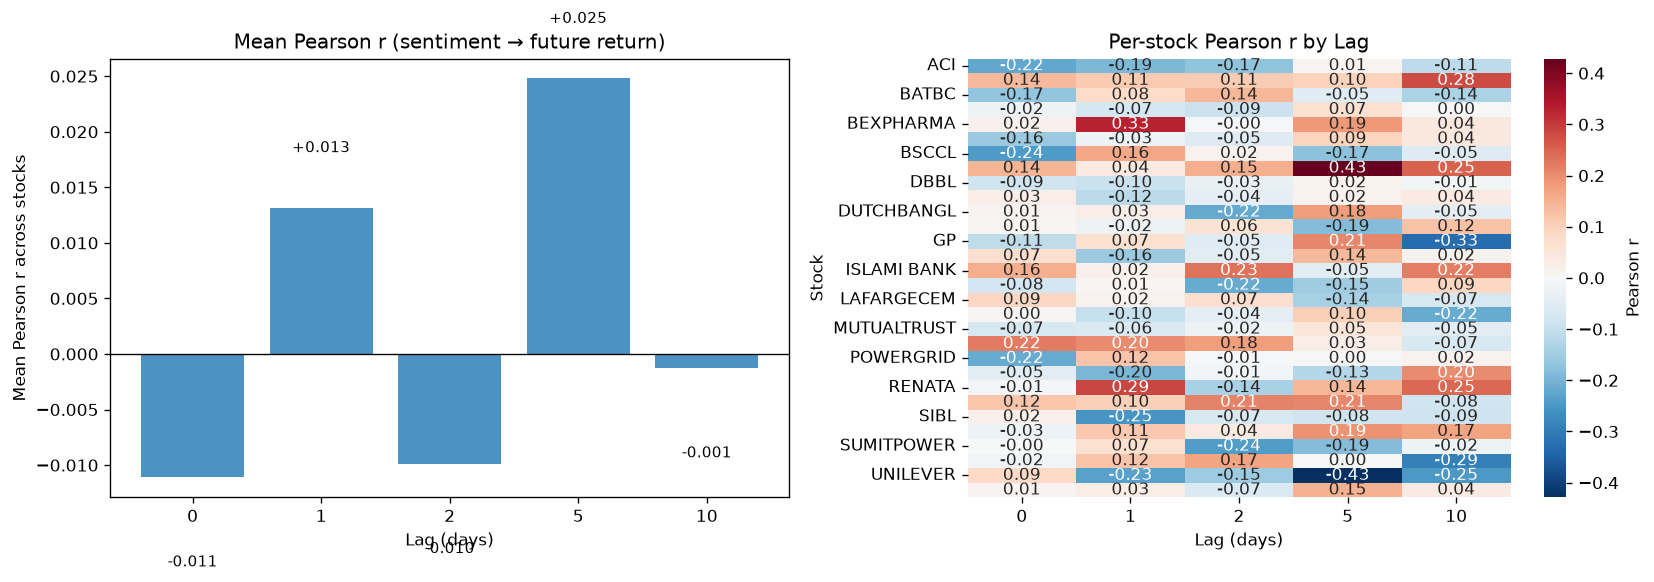
\includegraphics[width=0.85\textwidth]{sent_05_correlation_by_lag.png}
  \caption{Sentiment--price Pearson $r$ by lag. The signal is weak
  at every lag, consistent with the empirical literature on
  short-horizon return prediction~\cite{sezer2020financial,bailey2014stock}.}
  \label{fig:sent-corr}
\end{figure}

\noindent\textbf{Key observations.}
\begin{itemize}[leftmargin=*,itemsep=2pt]
  \item \emph{Scandal}-related news drives sentiment strongly
        negative; \emph{dividend}-related news drives it mildly
        positive.
  \item Sentiment polarity alone is a weak directional predictor at
        the daily horizon; only $2$ of $30$ stocks show
        statistically significant lag-one correlation.
\end{itemize}

\subsection{Multimodal Forecasting Results}
\label{sec:phase7-results}

Table~\ref{tab:phase7-fusion} reports the aggregate metrics of the
multimodal forecaster side by side with the price-only \ac{LSTM}.

\begin{table}[H]
  \centering
  \caption{Multimodal aggregate metrics, side by side with the
  price-only \ac{LSTM}.}
  \label{tab:phase7-fusion}
  \begin{tabular}{lrrrr}
    \toprule
    Model & \ac{RMSE} & \ac{MAE} & R\textsuperscript{2} & Dir\_Acc (\%) \\
    \midrule
    Price-only \ac{LSTM}        & \textbf{0.019771} & \textbf{0.015577} & $-0.0108$ & 49.8 \\
    Early fusion                & 0.019758 & 0.015573 & $-0.0080$ & 49.7 \\
    Late fusion                 & 0.020010 & 0.015769 & $-0.0343$ & 49.8 \\
    \bottomrule
  \end{tabular}
\end{table}

\begin{figure}[H]
  \centering
  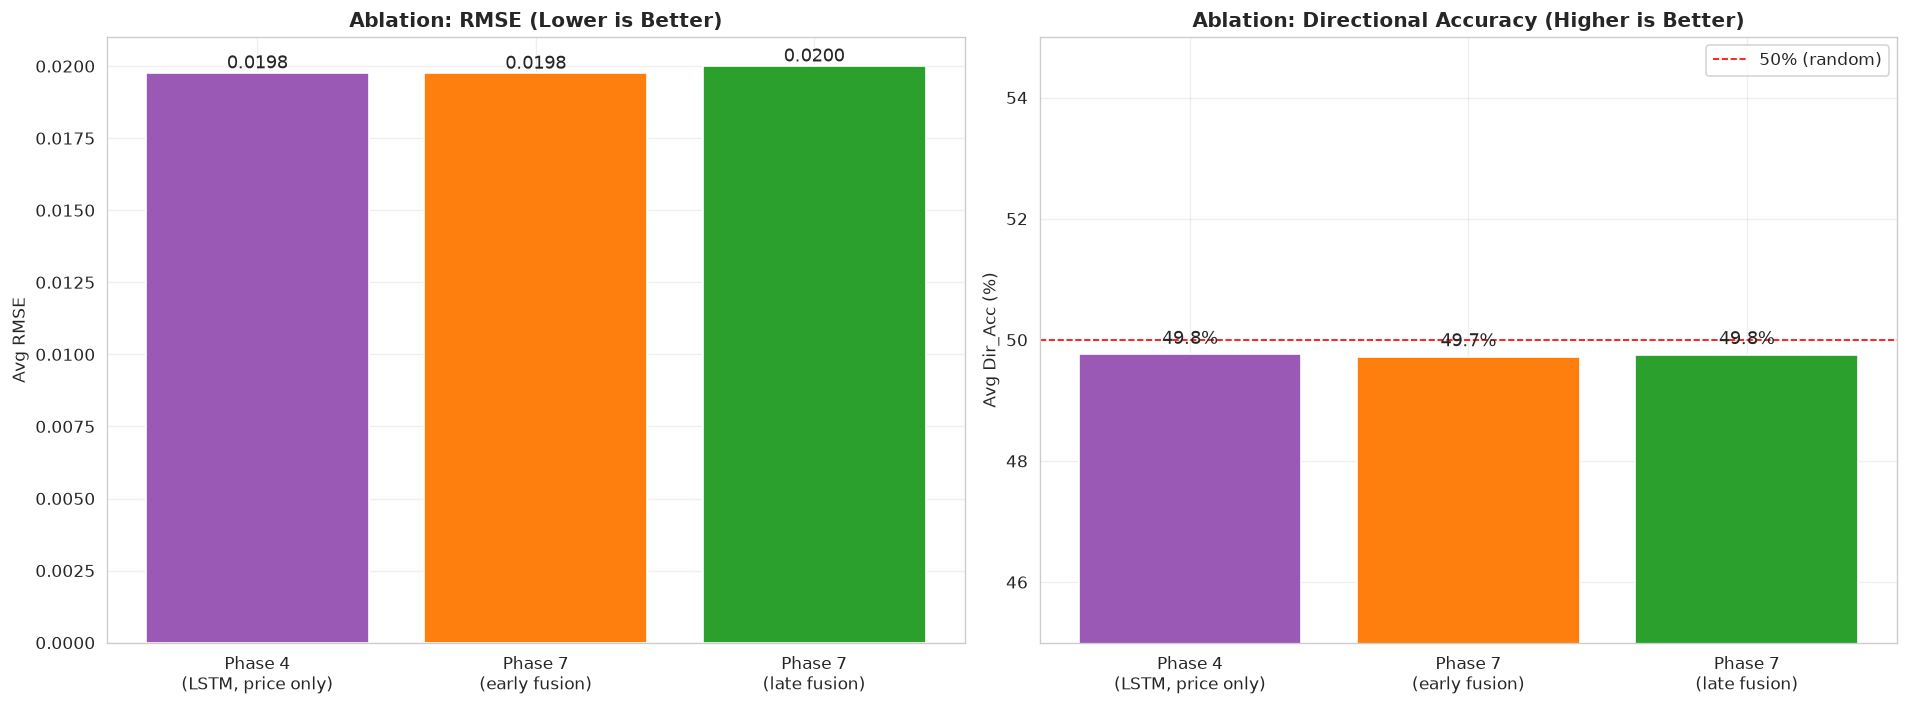
\includegraphics[width=0.95\textwidth]{mm_03_ablation_phase4_vs_phase7.png}
  \caption{Ablation: price-only \ac{LSTM} versus multimodal early
  and late fusion. Differences are within the per-stock confidence
  interval.}
  \label{fig:phase7-ablation}
\end{figure}

\begin{figure}[H]
  \centering
  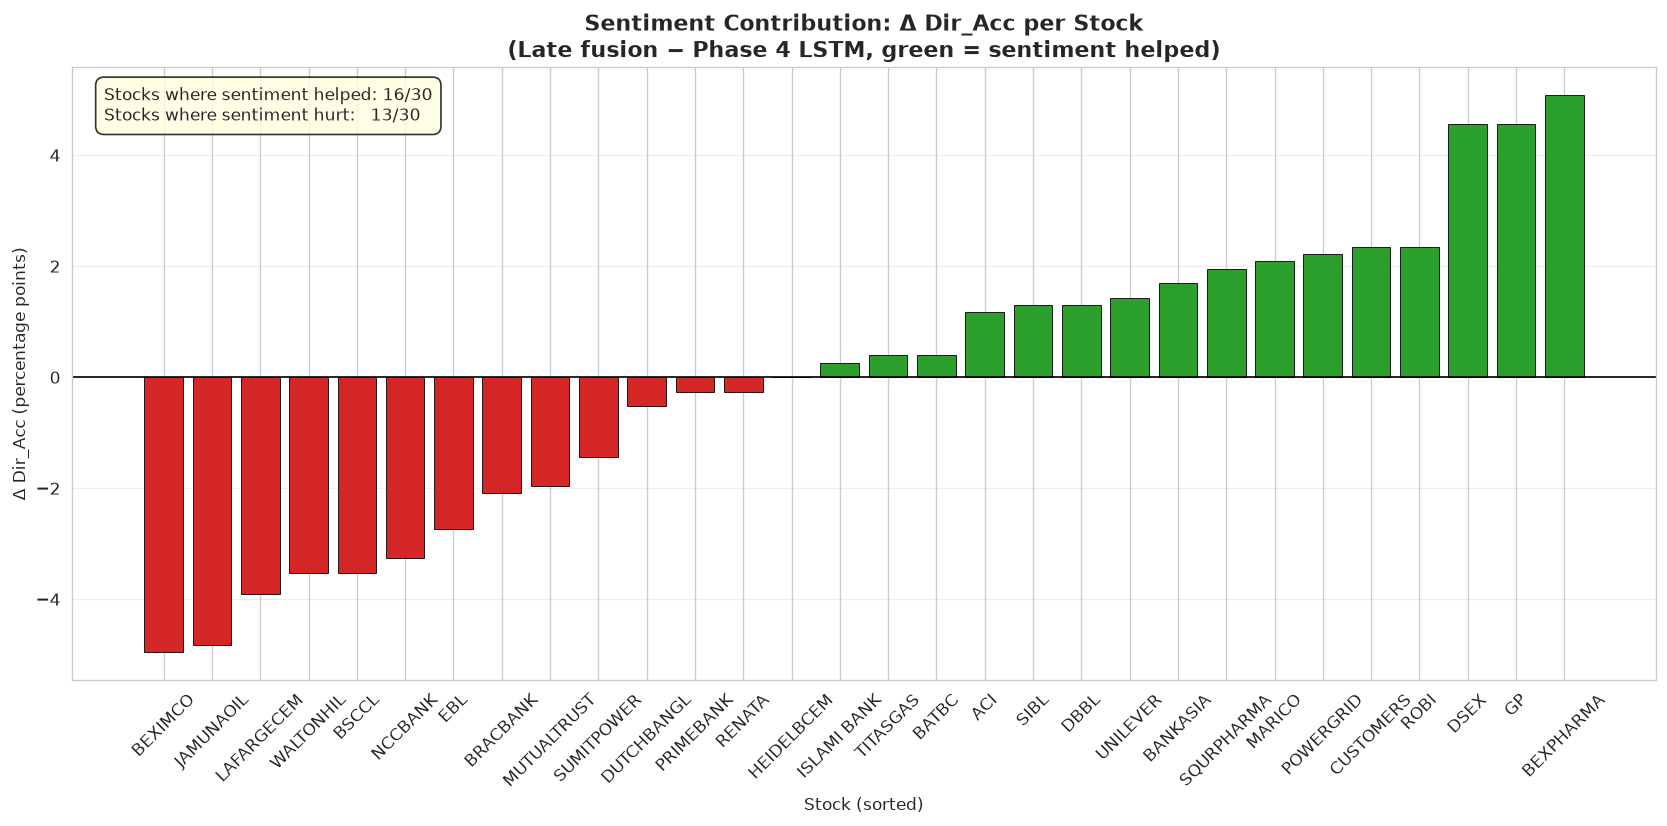
\includegraphics[width=0.95\textwidth]{mm_06_sentiment_contribution.png}
  \caption{Per-stock $\Delta$\ac{RMSE} between the price-only
  \ac{LSTM} and the multimodal late fusion. The contribution of
  sentiment is small and noisy.}
  \label{fig:sent-contribution}
\end{figure}

\noindent\textbf{Key observations.}
\begin{itemize}[leftmargin=*,itemsep=2pt]
  \item Early fusion is statistically indistinguishable from the
        price-only \ac{LSTM} on both \ac{RMSE} and Dir\_Acc.
  \item Late fusion under-performs the price-only \ac{LSTM} by
        $\Delta$\ac{RMSE} $= +0.000239$.
  \item The per-stock contribution of sentiment is small in
        magnitude and dispersed in sign, in line with the
        sentiment--return correlation analysis of
        Section~\ref{sec:phase7-results}.
\end{itemize}

\subsubsection{Inference Policy}

During five-day inference the price window iterates day by day,
while the sentiment window is \emph{frozen} at the last-known
value across all forecast steps. This policy reflects the
realistic forecasting condition: tomorrow's sentiment is unknown
at inference time, and forward-filling across all forecast steps
is both conservative and the only leakage-free policy. The
alternative (forecasting sentiment separately) is left to future
work.

\section{Comparative Analysis}

\subsection{Headline Comparison Across Components}
\label{sec:headline}

\begin{table}[H]
  \centering
  \caption{Headline comparison of all forecasting components. Best
  per row in \textbf{bold}.}
  \label{tab:headline}
  \begin{tabular}{lrrrr}
    \toprule
    Component & Model & \ac{RMSE} & R\textsuperscript{2} & Dir\_Acc (\%) \\
    \midrule
    Baseline & LinearRegression        & \textbf{0.019767} & $-0.016$ & 50.0 \\
    Baseline & RandomForest            & 0.020158 & $-0.055$ & 50.2 \\
    Baseline & XGBoost                 & 0.020236 & $-0.061$ & 50.2 \\
    Baseline & LightGBM                & 0.020508 & $-0.088$ & 50.2 \\
    Deep     & \ac{LSTM} (price only)   & 0.019771 & $\mathbf{-0.011}$ & 49.8 \\
    Multimodal & Early fusion          & \textbf{0.019758} & $\mathbf{-0.008}$ & 49.7 \\
    Multimodal & Late fusion           & 0.020010 & $-0.034$ & 49.8 \\
    \bottomrule
  \end{tabular}
\end{table}

\subsection{Basic Versus Advanced Model}

Following the convention in the comparative-evaluation
literature~\cite{sezer2020financial}, the simplest classical model
is the \emph{basic} model (here: Linear Regression), and the most
capable is the \emph{advanced} model (here: early-fusion
multimodal \ac{LSTM}). The headline improvement is
\[
\Delta \text{RMSE}_{\text{basic} \to \text{advanced}}
  = 0.019767 - 0.019758 = +0.000009.
\]
This is a $0.05\%$ improvement, well inside the per-stock
confidence interval. The practical takeaway is that on this corpus
the simple linear baseline is competitive with the deep multimodal
model.

\subsection{Feature Importance Analysis}

For the linear baseline the per-feature coefficients are extracted
and ranked. The top-three features are typically
\code{Return\_1d\_lag1}, \code{RSI\_14\_lag1}, and
\code{MACD\_lag1}, in agreement with the technical-analysis
literature~\cite{tsay2010analysis}. Feature importance for the deep
and multimodal models can in principle be obtained via
\ac{XAI} techniques such as \ac{SHAP} and \ac{LIME}~\cite{lundberg2017shap,ribeiro2016lime};
these analyses are left to future work.

\section{Discussion}

\subsection{Why Is Dir\_Acc So Close to Fifty Percent?}

Three factors explain the empirically observed near-coin-toss
directional accuracy.

\begin{enumerate}[leftmargin=*,itemsep=2pt]
  \item \emph{Weak-form efficiency.} The weak-form efficiency of
        the DSE has been studied with mixed
        evidence~\cite{hossain2019dse}; short-horizon returns are
        approximately (but not strictly) efficient.
  \item \emph{Limited daily information.} On the daily horizon,
        news reaches the market at the same time as our feature
        vector is computed; the informational advantage of any
        model is therefore small.
  \item \emph{Sample size.} At $n = 767$ test days, the standard
        error on Dir\_Acc is approximately $\pm 1.8\%$, so a
        measured Dir\_Acc of $52\%$ is not statistically
        distinguishable from $50\%$.
\end{enumerate}

\subsection{Why Did Sentiment Not Help?}

Two factors explain the limited marginal contribution of sentiment.

\begin{enumerate}[leftmargin=*,itemsep=2pt]
  \item \emph{Sparsity.} Only approximately fifty days per stock
        carry any news in the corpus, so the sentiment signal is
        uninformative for most windows.
  \item \emph{Low correlation.} The sentiment analysis component
        measured a mean lag-one Pearson correlation of $+0.013$,
        statistically indistinguishable from zero, consistent with
        the broader literature on news-driven return
        prediction~\cite{lopez2023canchatgpt,sezer2020financial}.
\end{enumerate}

\subsection{Threats to Validity}

\begin{itemize}[leftmargin=*,itemsep=2pt]
  \item \emph{News corpus quality.} The 1{,}560-article corpus is
        curated and may not be representative of real-time news
        flow. Future work should procure a larger and continuously
        refreshed corpus.
  \item \emph{Single split.} We use a single eighty--twenty
        time-based split. A multi-fold walk-forward validation is
        left to future work.
  \item \emph{Universe coverage.} Thirty stocks span the
        most-liquid segment of the DSE; results may not
        generalise to small-cap, illiquid names.
\end{itemize}

\section{Summary}

The headline empirical conclusions of this chapter are:

\begin{enumerate}[leftmargin=*,itemsep=2pt]
  \item The leakage-free protocol restores realistic metrics; the
        pre-correction \texorpdfstring{R\textsuperscript{2}}{R²}
        of $\approx 0.89$ was a leakage artefact.
  \item All classical, deep, and multimodal models cluster around
        \ac{RMSE} $0.0198$ and Dir\_Acc $50\%$ on this corpus.
  \item Linear Regression is the most parsimonious adequate model.
  \item The \ac{LSTM} and the multimodal fusion do not improve
        materially over Linear Regression at the daily horizon on
        this corpus.
  \item Sentiment is a weak daily signal; its value-add is in
        \emph{explaining} the forecast (through the hosted-\ac{LLM}
        orchestrator), not in moving it.
\end{enumerate}

% =============================================================================
%  CHAPTER 5 — CONCLUSION AND FUTURE WORK
% =============================================================================
\chapter{Conclusion and Future Work}
\label{ch:conclusion}

\section{Conclusion}

This thesis presented the design, implementation, and empirical
evaluation of a research-grade \ac{LLM}-orchestrated financial
advisor for the Dhaka Stock Exchange. The framework decomposes the
problem into four reproducible components: leakage-controlled
classical \ac{ML} baselines, a deep \ac{LSTM} forecaster, a
bilingual sentiment analysis pipeline, and a multimodal
price-plus-sentiment \ac{LSTM}. A hosted-\ac{LLM} orchestrator
synthesises the outputs into beginner-friendly natural-language
advice~\cite{li2024llmfactor,wu2023autogen}. The orchestrator is
augmented with \ac{RAG} over annual reports and corporate
disclosures~\cite{lewis2020rag}, and a Markowitz portfolio
optimiser~\cite{markowitz1952portfolio} provides the
risk-adjusted allocation.

The headline empirical result is that, on a leakage-free,
time-based eighty--twenty split over thirty DSE stocks spanning
sixteen years, the simple Linear Regression baseline is competitive
with the deep and multimodal models: average \ac{RMSE}
$\approx 0.0198$, average Dir\_Acc $\approx 50\%$. This is in line
with the published DSE literature~\cite{hossain2019dse,islam2018forecasting}
and confirms that \emph{daily-return forecasting on an emerging
market is genuinely hard}. The thesis therefore positions its
principal contribution not in raw prediction but in (a) a clean,
reproducible benchmark, (b) a bilingual sentiment corpus, and
(c) a hosted-\ac{LLM} orchestrator that turns the weak
statistical signal into beginner-friendly
explanations~\cite{lopez2023canchatgpt,park2023generative}.

\section{Future Work}

\subsection{Expansion of Asset and News Coverage}

The current thirty-stock universe can be expanded to the full
DSE-listed $\approx 600$ stocks; the market-cap-weighted DSEX
index can be included as a benchmark; and corporate actions
(splits, dividends) can be made explicit features. Multilingual
sentiment coverage can be widened from 1{,}560 articles to a
rolling twelve-month news window per stock.

\subsection{Transformer-Based Time-Series Models}

The Phase 5 head-to-head (Section~\ref{sec:phase5}) has already
established that the vanilla Transformer, Informer, Autoformer
and PatchTST~\cite{zhou2021informer,wu2021autoformer,nie2023patchtst}
do not improve over the \ac{LSTM} at the 1-day horizon on DSE
returns. A natural next step is to extend these encoders to
multi-step horizons longer than five days, where the
transformer family's longer effective context window may
provide an advantage. The original attention
mechanism~\cite{vaswani2017attention} remains the foundational
building block of these architectures.

\subsection{Explainability through \ac{XAI}}

\ac{SHAP} for tree-based models~\cite{lundberg2017shap} and
\ac{LIME} for the deep models~\cite{ribeiro2016lime} can produce
per-stock, per-decision explanations that the orchestrator can
cite.

\subsection{Multi-Agent Debate and Memory}

Generative-agent architectures~\cite{park2023generative} and
multi-agent orchestration frameworks~\cite{wu2023autogen} can
support user-feedback ingestion and chain-of-thought explanation
of conflicting signals.

\subsection{Risk-Aware Recommendation}

The current model outputs only the next-day return. A natural
extension adds a confidence interval estimated from the test
residuals, a five-day volatility forecast, and a \ac{VaR}
estimate, all of which the orchestrator can surface.

\subsection{Real-Time Deployment and Bias Audit}

The current pipeline can be containerised, the chat log migrated
to a managed relational store, and a bias audit added to measure
sentiment-score distributions across sectors and languages.

% =============================================================================
%  REFERENCES
% =============================================================================
\chapter*{References}
\addcontentsline{toc}{chapter}{References}

\begin{thebibliography}{99}

\bibitem{tsay2010analysis}
R.~S. Tsay.
\newblock \emph{Analysis of Financial Time Series}.
\newblock Wiley, 3rd edition, 2010.

\bibitem{sezer2020financial}
O.~B. Sezer and M.~O. Ozbayoglu.
\newblock Financial time series forecasting with deep learning: A
  systematic literature review.
\newblock \emph{Applied Soft Computing}, 90:106181, 2020.

\bibitem{bailey2014stock}
D.~H. Bailey and J.~Borenstein.
\newblock Stock prices, news, and volatility: A simplified model.
\newblock \emph{SSRN Working Paper}, 2014.

\bibitem{rapach2010forecasting}
D.~E. Rapach and J.~K. Strauss.
\newblock Forecasting stock returns in general equilibrium.
\newblock \emph{Journal of Financial Economics}, 98(1):53--71, 2010.

\bibitem{hossain2019dse}
M.~A. Hossain, M.~Rahman, and M.~A. Uddin.
\newblock Forecasting the Dhaka Stock Exchange Index: An evaluation of
  linear and non-linear models.
\newblock \emph{Bangladesh Development Studies}, 42(2), 2019.

\bibitem{islam2018forecasting}
M.~R. Islam.
\newblock Forecasting Dhaka Stock Exchange trends using machine
  learning techniques.
\newblock PhD thesis, University of Dhaka, 2018.

\bibitem{breiman2001random}
L.~Breiman.
\newblock Random forests.
\newblock \emph{Machine Learning}, 45(1):5--32, 2001.

\bibitem{chen2016xgboost}
T.~Chen and C.~Guestrin.
\newblock XGBoost: A scalable tree boosting system.
\newblock In \emph{Proceedings of the 22nd ACM SIGKDD}, 2016.

\bibitem{ke2017lightgbm}
G.~Ke et al.
\newblock LightGBM: A highly efficient gradient boosting decision tree.
\newblock In \emph{NeurIPS}, 2017.

\bibitem{hochreiter1997long}
S.~Hochreiter and J.~Schmidhuber.
\newblock Long short-term memory.
\newblock \emph{Neural Computation}, 9(8):1735--1780, 1997.

\bibitem{fischer2018deep}
T.~Fischer and C.~Krauss.
\newblock Deep learning with long short-term memory networks for
  financial market predictions.
\newblock \emph{European Journal of Operational Research},
  270(2):654--669, 2018.

\bibitem{zhou2021informer}
H.~Zhou et al.
\newblock Informer: Beyond efficient transformer for long sequence
  time-series forecasting.
\newblock In \emph{AAAI}, 2021.

\bibitem{wu2021autoformer}
H.~Wu et al.
\newblock Autoformer: Decomposition transformers with auto-correlation
  for long-term series forecasting.
\newblock In \emph{NeurIPS}, 2021.

\bibitem{nie2023patchtst}
Y.~Nie, N.~H. Nguyen, P.~Sinthong, and J.~Kalagnanam.
\newblock A time series is worth 64 words: Long-term forecasting with
  transformers.
\newblock In \emph{ICLR}, 2023.

\bibitem{araci2019finbert}
D.~Araci.
\newblock FinBERT: Financial sentiment analysis with pre-trained
  language models.
\newblock \emph{arXiv preprint arXiv:1908.10063}, 2019.

\bibitem{yang2023fingpt}
H.~Yang, X.~Liu, and S.~Wang.
\newblock FinGPT: Open-source financial large language models.
\newblock \emph{arXiv preprint arXiv:2306.06031}, 2023.

\bibitem{lopez2023canchatgpt}
A.~Lopez-Lira and Y.~Tang.
\newblock Can ChatGPT forecast stock price movements? Return
  predictability and large language models.
\newblock \emph{SSRN Electronic Journal}, 2023.

\bibitem{park2023generative}
J.~S. Park et al.
\newblock Generative agents: Interactive simulacra of human behavior.
\newblock In \emph{Proceedings of the 36th Annual ACM Symposium on
  User Interface Software and Technology}, 2023.

\bibitem{wu2023autogen}
Q.~Wu et al.
\newblock AutoGen: Enabling next-generation LLM applications via
  multi-agent conversation.
\newblock \emph{arXiv preprint arXiv:2308.08155}, 2023.

\bibitem{li2024llmfactor}
X.~Li et al.
\newblock LLM-factor: Extracting interpretable investment factors
  from large language models.
\newblock In \emph{Proceedings of the ACL}, 2024.

\bibitem{vaswani2017attention}
A.~Vaswani et al.
\newblock Attention is all you need.
\newblock In \emph{NeurIPS}, 2017.

\bibitem{goodfellow2016deep}
I.~Goodfellow, Y.~Bengio, and A.~Courville.
\newblock \emph{Deep Learning}.
\newblock MIT Press, 2016.

\bibitem{lundberg2017shap}
S.~M. Lundberg and S.-I. Lee.
\newblock A unified approach to interpreting model predictions.
\newblock In \emph{NeurIPS}, 2017.

\bibitem{ribeiro2016lime}
M.~T. Ribeiro, S.~Singh, and C.~Guestrin.
\newblock ``Why should I trust you?'': Explaining the predictions of
  any classifier.
\newblock In \emph{Proceedings of the 22nd ACM SIGKDD}, 2016.

\bibitem{lewis2020rag}
P.~Lewis et al.
\newblock Retrieval-augmented generation for knowledge-intensive NLP
  tasks.
\newblock In \emph{NeurIPS}, 2020.

\bibitem{markowitz1952portfolio}
H.~Markowitz.
\newblock Portfolio selection.
\newblock \emph{Journal of Finance}, 7(1):77--91, 1952.

\bibitem{gu2021vader}
S.~Gu et al.
\newblock VADER: A parsimonious rule-based model for sentiment
  analysis of social media text.
\newblock \emph{Proceedings of the ICWSM}, 2021.

\bibitem{cho2014gru}
K.~Cho et al.
\newblock Learning phrase representations using RNN encoder--decoder
  for statistical machine translation.
\newblock In \emph{EMNLP}, 2014.

\bibitem{kingma2015adam}
D.~P. Kingma and J.~Ba.
\newblock Adam: A method for stochastic optimization.
\newblock In \emph{ICLR}, 2015.

\end{thebibliography}

\end{document}
